\documentclass[titlepage]{article}
\usepackage[utf8]{inputenc}
\usepackage{setspace}
\usepackage[left=1in, right=1in, top=1in, bottom=1in]{geometry}
\usepackage{verbatim}
\usepackage{fancyhdr}
\usepackage{float}
\usepackage{matlab-prettifier}
\usepackage{amssymb}
\usepackage{amsmath}
\usepackage{mathtools}
\usepackage{blindtext}
\usepackage{textcomp}

\usepackage{stackengine}
\stackMath

\usepackage{graphicx}
\graphicspath{ {./figures/} }

\usepackage{xcolor}

\definecolor{codegreen}{rgb}{0,0.6,0}
\definecolor{codegray}{rgb}{0.5,0.5,0.5}
\definecolor{codepurple}{rgb}{0.58,0,0.82}
\definecolor{backcolour}{rgb}{0.95,0.95,0.92}

\lstdefinestyle{mystyle}{
    backgroundcolor=\color{backcolour},   
    commentstyle=\color{codegreen},
    keywordstyle=\color{magenta},
    numberstyle=\tiny\color{codegray},
    stringstyle=\color{codepurple},
    basicstyle=\ttfamily\footnotesize,
    breakatwhitespace=false,         
    breaklines=true,                 
    captionpos=b,                    
    keepspaces=true,                 
    numbers=left,                    
    numbersep=5pt,                  
    showspaces=false,                
    showstringspaces=false,
    showtabs=false,                  
    tabsize=2
}

\lstset{style=mystyle}

\singlespacing
\parindent=0in

\title{ME 577 Final Project}
\author{Charles Goble, Cory Anderson-Wilson, Andy Edgell, \& Eddie Turner}
\date{\today}
\cfoot{Page \thepage}

\begin{document}
\maketitle
\tableofcontents

\newpage
\section{Introduction}
The inverted pendulum on a cart problem is an interesting engineering problem for a multitude of reasons. It serves as the basis for both real and surrogate systems. Companies such as Segway\texttrademark{} have a self-balancing system marketed as a personal transportation device for urban environments. In this instance, the inverted pendulum on a cart has been actualized into a physical product and sold to the masses. However, the more common realization of the inverted pendulum on a cart problem is a surrogate model for a more complicated dynamical system. NASA has published research showing how the inverted pendulum on a cart problem acts as a rocket in flight and the derived controller can be used to design a control law for a launch vehicle[5]. Finally, the most widely used application of the inverted pendulum on a cart problem is in academia where academics mentor their students in a variety of controls topics using the non-stable but controllable dynamics system to highlight key concepts in controls engineering.\\

This report follows in the latter example of the utilization for the inverted pendulum on a cart. The inverted pendulum on a cart is the dynamical system for the University of Alabama ME 577: Advanced Linear Control course final project. Contained within this report, the reader will find a derivation and linearization of the dynamical system, two controller designs and finally some system response analysis testing the controllers.

\newpage
\section{Dynamics Derivation}
To start the derivation of the equations of motion, we first need to split the inverted pendulum on a cart into separate components and draw a free body diagram of each.

\begin{figure}[H]
\center
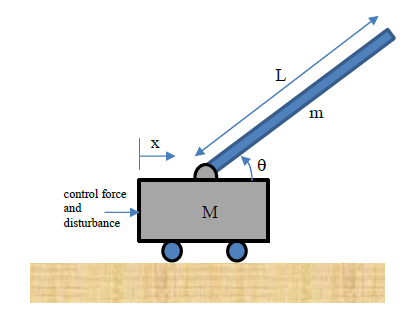
\includegraphics[width=5cm, height=5cm]{prompt_diagram.png}
\caption{Free Body Diagrams of Individual Components}
\end{figure}

\begin{figure}[H]
\center
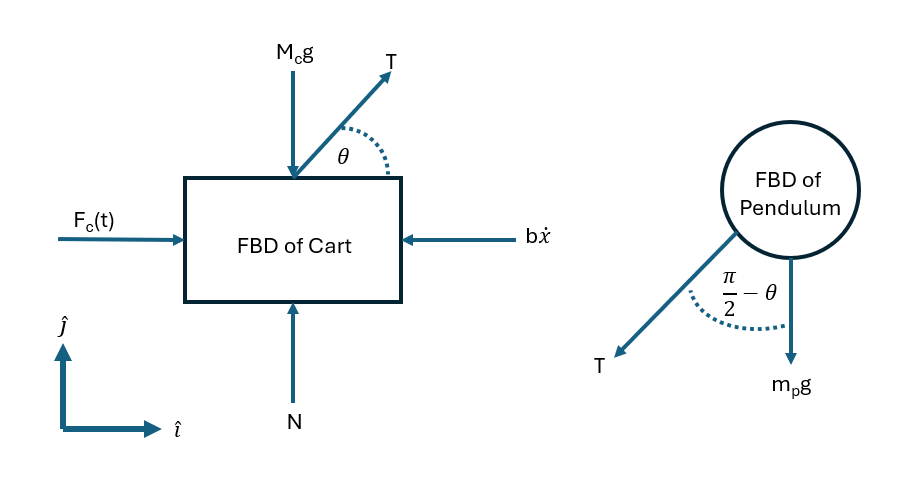
\includegraphics[width=1\linewidth]{free_body_diagram.png}
\caption{Free Body Diagrams of Individual Components}
\end{figure}

As shown in Figure 1, the individual forces act on the cart are the weight, an external control force, a friction damping force, the normal force from the road and a tension force from the rod connecting the pendulum to the cart. The only forces acting on the pendulum are the same rod tension force and the weight of the pendulum. The first step will be to sum all the forces along each coordinate axis for the cart and pendulum[2].\\

\underline{Cart Forces:}
\begin{equation}
\sum{}{F_{\hat{i}}} = f_{c}\left(t\right) = M_{c}\ddot{x} + b\dot{x} + T\cos{\theta}
\end{equation}
\[ \sum{}{F_{\hat{j}}} = f_{c}\left(t\right) = N - M_{c}g + - T\sin{\theta} = M_{c}\ddot{y}=0 \]

Since the cart is not able to travel in the \(\hat{j}\) direction, the second force summation equation for the cart is mainly shown for completeness. It will be unused in the derivation. If we were interested in quantifying the Normal force acting up on the cart from the road we would use it, however that is not necessary[2].\\

\underline{Pendulum Forces:}
\[ \sum{}{F_{\hat{i}}} = -T\cos{\theta} = m_{p}a_{p_{x}}\]
\[ \sum{}{F_{\hat{j}}} =  -T\sin{\theta} -m_{p}g = m_{p}a_{p_{y}} \]

In the pendulum equations, a new term has been identified, \(a_{p}\) which acts in both the \(\hat{i}\) and the \(\hat{j}\) directions. This is the acceleration of the pendulum and becomes a force when multiplied by the mass of the pendulum[2]. To compute the acceleration of the pendulum we will use the following equation:

\[a_p = a_c + a_{p/c}\]

where \(a_p\) is the desired acceleration of the pendulum, \(a_c\) is the acceleration of the cart and \(a_{p/c}\) is the acceleration of the pendulum relative to the cart. Defining the acceleration of the cart is easy, it is simply \(a_c=\ddot{x}\hat{i}\). To determine the relative acceleration, we need to use the transport theorem and place a rotating frame on the pendulum and map the acceleration back to our previously defined inertial frame.

\begin{figure}[H]
\center
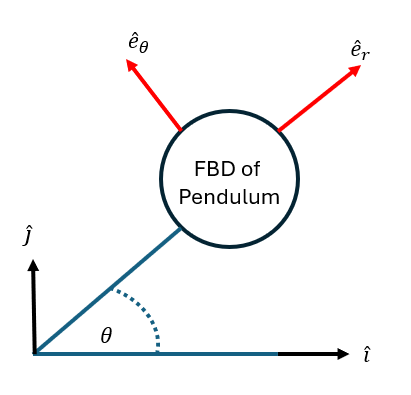
\includegraphics[width=5cm, height=5cm]{rotating_frame.png}
\caption{Pendulum Rotating Coordinate System}
\end{figure}

To compute the desired acceleration, we will use kinematics and start with a position definition for the pendulum in the rotating frame and then take two derivatives using the transport theorem to compute the relative acceleration back to the inertial frame[6].

\[r = L\hat{e_{r}}\]
\[\dot{r}^{n} = \dot{r}^{b} + \omega_{p/c} \times r = L\dot{\theta}\hat{e_{\theta}}\]
\[\ddot{r}^{n} = \ddot{r}^{b} + \omega_{p/c} \times \dot{r} = L\ddot{\theta}\hat{e_{\theta}} - L\dot{\theta}^{2}\hat{e_{r}}\]

We now have the relative acceleration of the pendulum to the cart in the pendulum's rotating frame. It is a simple transformation to go from the rotating polar coordinate system to the inertial cartesian coordinate system.
\[\hat{e_{r}} = \cos{\theta} \hat{i} + \sin{\theta} \hat{j}\]
\[\hat{e_{\theta}} = -\sin{\theta} \hat{i} + \cos{\theta} \hat{j}\]

Bringing all this together yields the following equation for the acceleration of the pendulum

\begin{equation}
a_p = \left[\ddot{x} -L\ddot{\theta}\sin{\theta} - L\dot{\theta}^{2}\right]\hat{i} + \left[L\ddot{\theta} - L\dot{\theta}\sin{\theta}\right]\hat{j}
\end{equation}

Equation two will now be inserted into the previously defined equations for the pendulum.

\begin{equation}
\sum{}{F_{\hat{i}}} = -T\cos{\theta} = m_{p}\ddot{x} - m_{p}L\ddot{\theta}\sin{\theta} - m_{p}L\dot{\theta}^{2}\cos{\theta}
\end{equation}

\begin{equation}
\sum{}{F_{\hat{j}}} = -T\sin{\theta} - m_{p}g = m_{p}L\ddot{\theta}\cos{\theta} - m_{p}L\dot{\theta}^{2}\sin{\theta}
\end{equation}

As you can see, equations one, three and four all have a variable T representing the tension force between the connecting rod for the cart and pendulum. We need to remove this variable from the equations. To do this, we will first multiply equation (3) by \(\sin{\theta}\) and equation (4) by \(\cos{\theta}\) and then subtract the two equations.

\[-T\cos{\theta}\sin{\theta} = m_{p}\ddot{x}\sin{\theta} - m_{p}L\ddot{\theta}\sin{\theta}^2 - m_{p}L\dot{\theta}^{2}\cos{\theta}\sin{\theta}\]
\[-T\sin{\theta}\cos{\theta} - m_{p}g\cos{\theta} = m_{p}L\ddot{\theta}\cos{\theta}^2 - m_{p}L\dot{\theta}^{2}\cos{\theta}\sin{\theta}\]

\begin{equation}
m_{p}g\cos{\theta} = m_{p}\ddot{x}\sin{\theta} - m_{p}L\ddot{\theta}
\end{equation}

To remove the tension force from equation (1), we will use the tension force found in equation three and substitute it into equation one.

\begin{equation}
T\cos{\theta} = M_{p}L\ddot{\theta}\sin{\theta} + m_{p}L\dot{\theta}^{2}\cos{\theta} - m_{p}\ddot{x}
\end{equation}

Substituting (6) into (1):
\[ f_{c}\left(t\right) = M_{c}\ddot{x} + b\dot{x} +  m_{p}L\ddot{\theta}\sin{\theta} + m_{p}L\dot{\theta}^{2}\cos{\theta} - m_{p}\ddot{x}\]

\begin{equation}
f_{c}\left(t\right) = \left[m_{p} + M_{c}\right]\ddot{x} + b\dot{x} -  m_{p}L\ddot{\theta}\sin{\theta} - m_{p}L\dot{\theta}^{2}\cos{\theta}
\end{equation}

Equations (5) and (7) are the governing non-linear equations of motion in differential form.

\subsection{Linearization}

To start the linearization process, we want to pick one of the two equilibrium conditions for this system. The equilibrium condition of interest, and the unstable but controllable condition, is when the pendulum is vertical at an angle of \(\theta = \pi / 2\).

We are going to now investigate what happens when a small perturbation happens around the equilibrium point.

\[\theta = \frac{\pi}{2} + \Delta\theta\]
\[\cos{\theta} = \cos{\left(\frac{\pi}{2} + \Delta\theta\right)} \approx \Delta\theta\]
\[\sin{\theta} = \sin{\left(\frac{\pi}{2} + \Delta\theta\right)} \approx 1\]

We choose to neglect any squared angle rate term because it will be sufficiently small and always close to zero.

\[\dot{\theta}^{2} \approx 0\]

Implementing these linearization techniques into equation (5) leads to the following set of coupled linear differential equations.

\[m_{p}g\theta = m_{p}\ddot{x} - m_{p}\ddot{\theta}\]
\begin{equation}
\ddot{\theta} = \frac{g}{L}\theta - \frac{1}{L}\ddot{x}
\end{equation}

Similarly, the same linearization process is done on equation (7).

\[\left[m_{p} + M_{c}\right] \ddot{x} = f_{c}\left(t\right) + m_{p}L\ddot{\theta} + b\dot{x}\]

\begin{equation}
\ddot{x} = \frac{b}{2m_{p} + M_{c}}\dot{x} + \frac{m_{p}g}{2m_{p} + M_{c}}\theta + \frac{1}{2m_{p} + M_{c}}f_{c}\left(t\right)
\end{equation}

Equation (9) represents the decoupled linear acceleration of the system. However, equation (8) which is the angular acceleration is still a function of the linear acceleration.
The desire is to express the accelerations only in terms of the state variables. Thus, we need to substitute equation (9) into equation (8) to remove the \(\ddot{x}\) term.

\begin{equation}
\ddot{\theta} = -\frac{b}{L\left(2m_{p} + M_{c}\right)}\dot{x} + \left[\frac{g}{L} - \frac{m_{p}g}{2m_{p} + M_{c}}\right]\theta - \frac{1}{L\left(2m_{p} + M_{c}\right)}f_{c}\left(t\right)
\end{equation}

We now have two equations (9) and (10) that represent the linearized decoupled dynamics of the system that are only a function of the state variables and the input control force.

\subsection{State Space Representation}

Using the equations developed up to this point, it is rather trivial to put the dynamical system into state space representation form.
Equation (11) and (12) show the state space representation as functions of time.

\begin{equation}
\begin{bmatrix}
\dot{x}\\
\ddot{x}\\
\dot{\theta}\\
\ddot{\theta}\\
\end{bmatrix} =
\begin{bmatrix}
0 & 1  & 0 & 0\\
0 & \frac{b}{2m_{p} + M_{c}}  & \frac{m_{p}g}{2m_{p} + M_{c}} & 0\\
0 & 0  & 0 & 1\\
0 & -\frac{b}{L\left(2m_{p} + M_{c}\right)}  & \frac{g}{L} - \frac{m_{p}g}{L\left(2m_{p} + M_{c}\right)} & 0\\
\end{bmatrix}
\begin{bmatrix}
x\\
\dot{x}\\
\theta\\
\dot{\theta}\\
\end{bmatrix}+ \begin{bmatrix}
0\\
\frac{1}{2m_{p} + M_{c}}\\
0\\
-\frac{1}{L\left(2m_{p} + M_{c}\right)}\\
\end{bmatrix} f_{c}\left(t\right)
\end{equation}

\begin{equation}
\vec{y}\left(t\right) = \begin{bmatrix}
1 & 0  & 0 & 0\\
0 & 1  & 0 & 0\\
0 & 0  & 1 & 0\\
0 & 0  & 0 & 1\\
\end{bmatrix} \begin{bmatrix}
x\\
\dot{x}\\
\theta\\
\dot{\theta}\\
\end{bmatrix} + \begin{bmatrix}
0\\
0\\
0\\
0\\
\end{bmatrix} f_{c}\left(t\right)
\end{equation}

Before showing the controller designs, it is meaningful to show the initial system response from equilibrium given a set of inital conditions and a small disturbance of a unit step or a unit impulse.

\begin{figure}[H]
\center
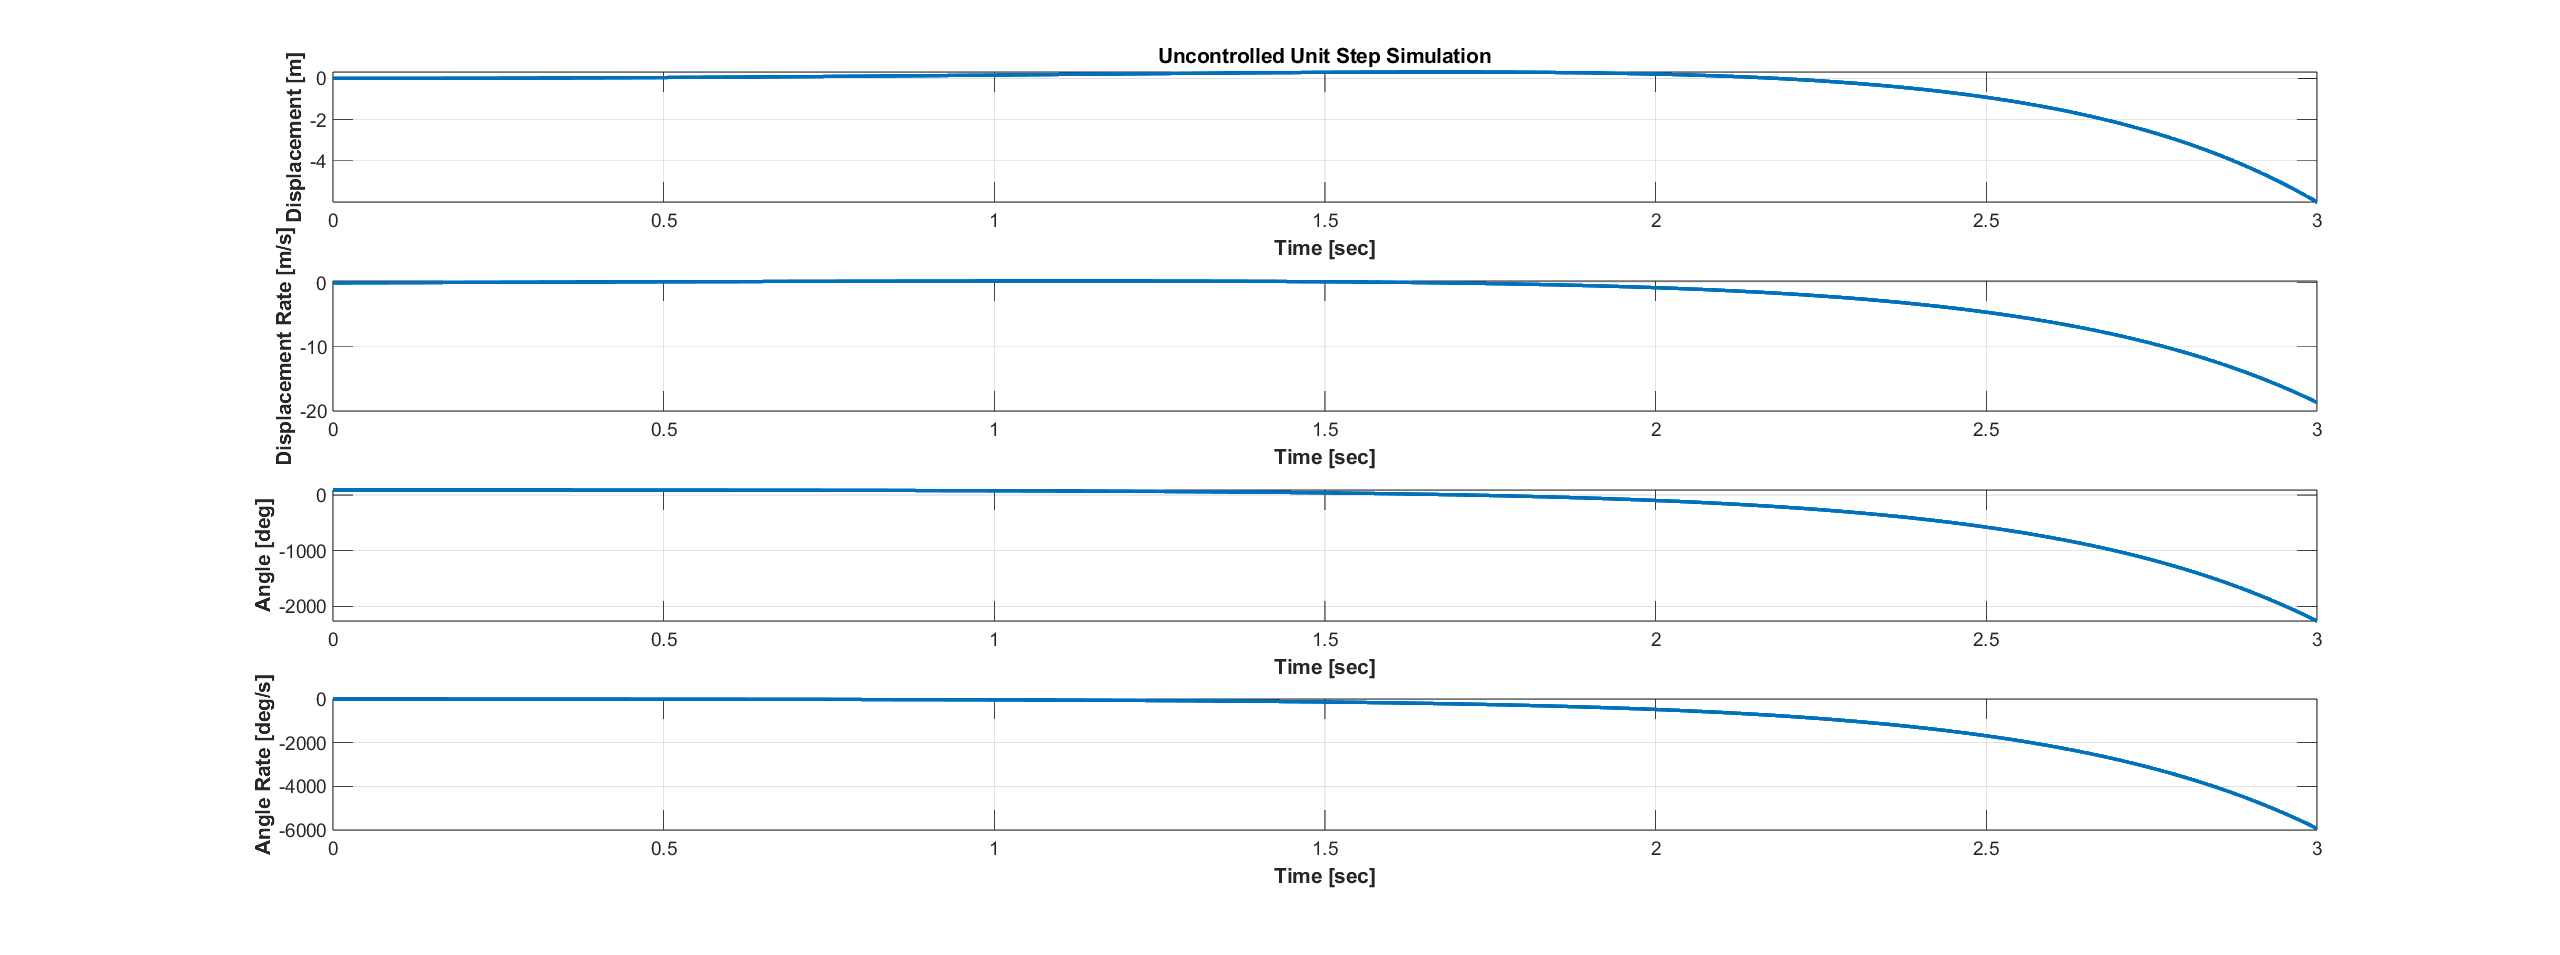
\includegraphics[width=1\linewidth]{uncontrolled_unit_step.png}
\caption{Uncontrolled Inverted Pendulum on Cart Unit Step Simulation}
\end{figure}

\begin{figure}[H]
\center
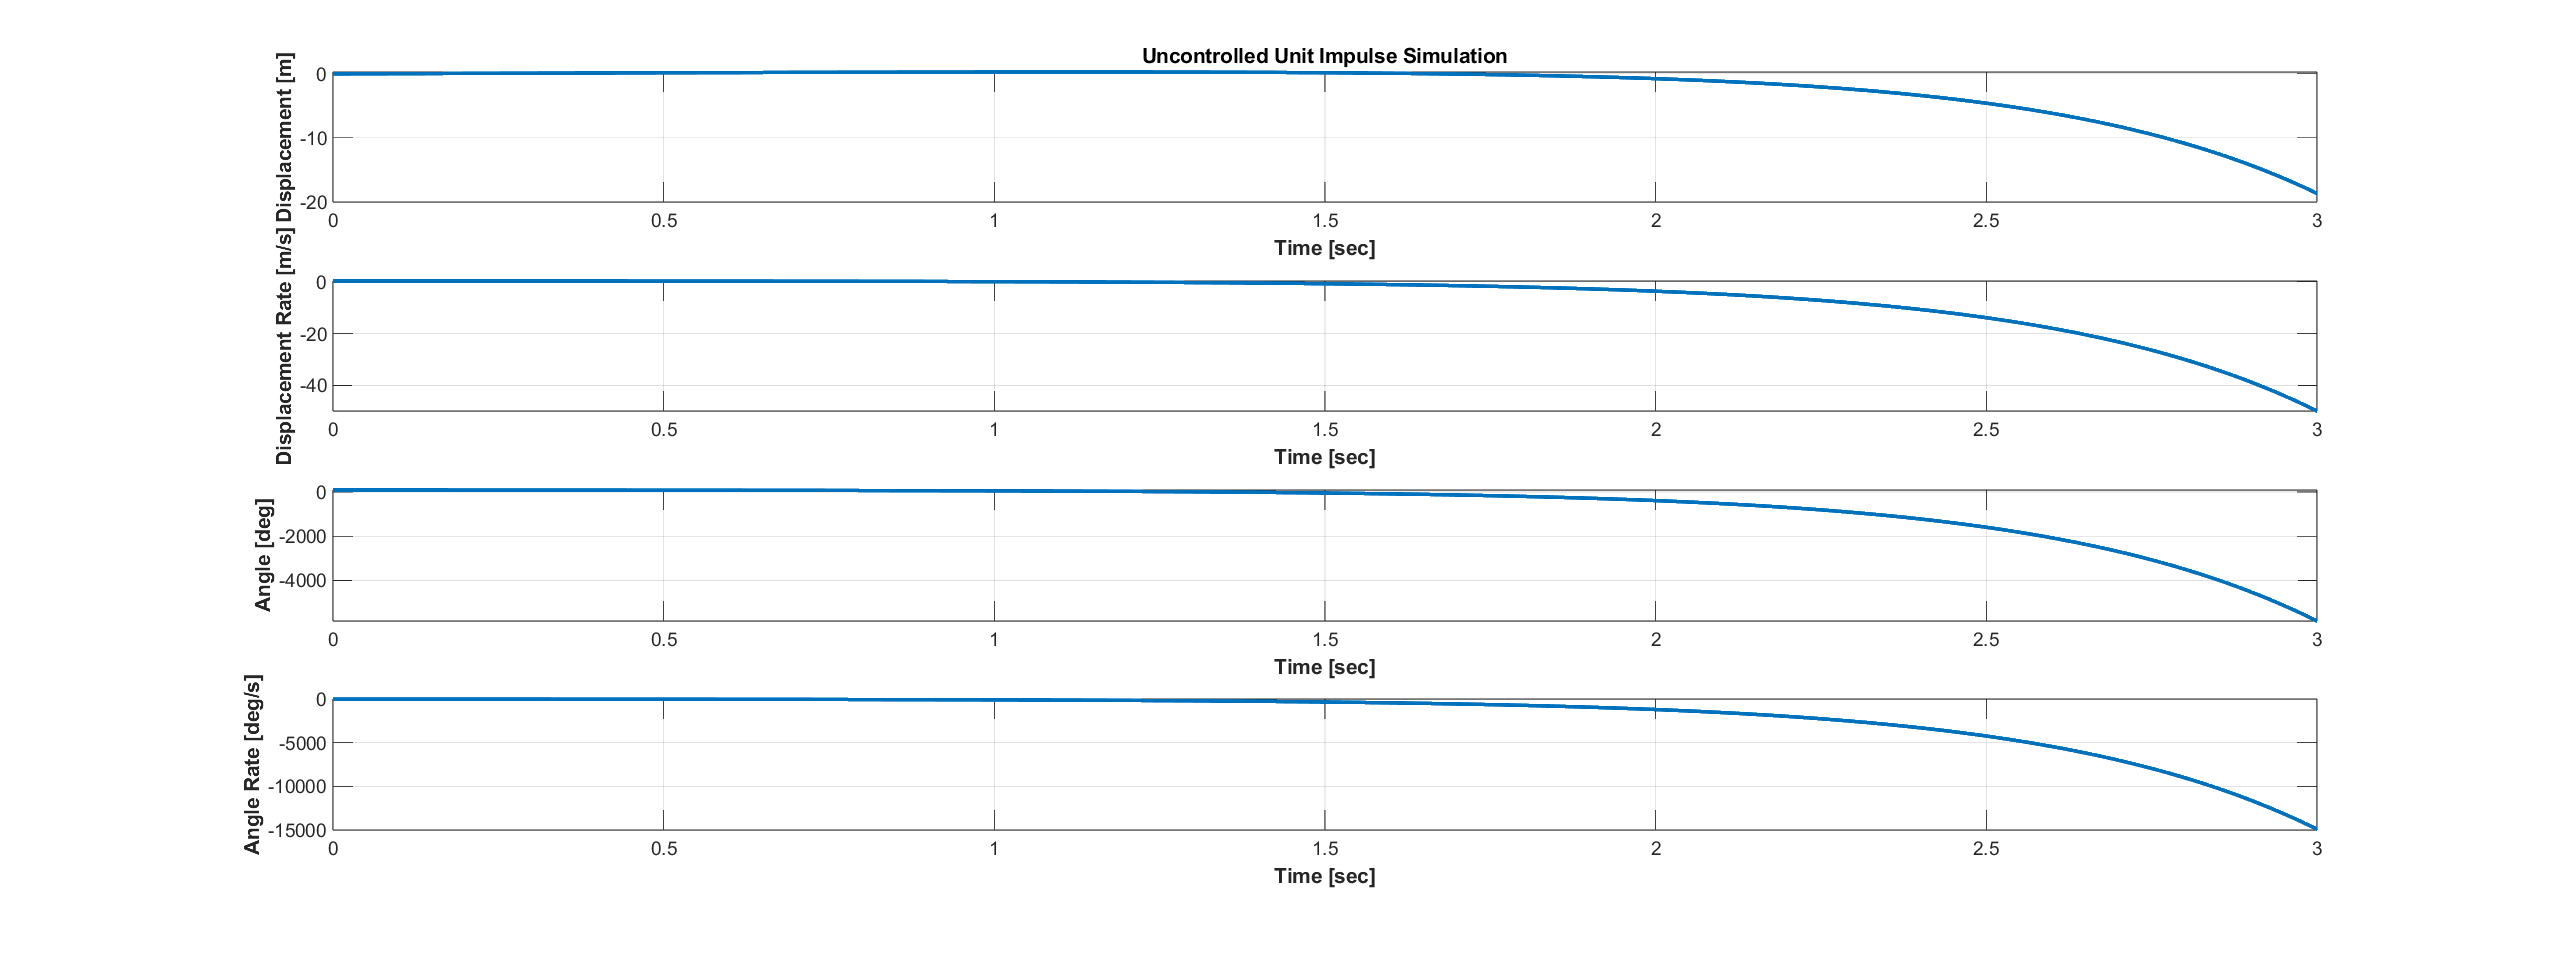
\includegraphics[width=1\linewidth]{uncontrolled_unit_impulse.png}
\caption{Uncontrolled Inverted Pendulum on Cart Unit Impulse Simulation}
\end{figure}

Figures 4 and 5 show that the motion diverges greatly after just a few seconds of simulation due to a unit disturbance. This demonstrates via simulation that the system is not stable and an active controller is necessary to stabilize the system.

Plugging in the values for the systems yeilds the following matrices:

\begin{equation}
	\textbf{A} = \begin{bmatrix}
		0 & 1 & 0 & 0\\
		0 & 0.0862 & 1.1828 & 0\\
		0 & 0 & 0 & 1\\
		0 & -0.0663 & 6.3557 & 0\\
		\end{bmatrix}
	\quad\quad\quad
	\textbf{B} = \begin{bmatrix}
		0 \\
		0.3448 \\
		0 \\
		-0.2653 \\
		\end{bmatrix}
	\quad\quad\quad
	\textbf{C} = \begin{bmatrix}
		1 & 0 & 0 & 0\\
		0 & 1 & 0 & 0\\
		0 & 0 & 1 & 0\\
		0 & 0 & 0 & 1\\
		\end{bmatrix}
	\quad\quad\quad
	\textbf{D} = \begin{bmatrix}
	0\\
	0\\
	0\\
	0\\
	\end{bmatrix}
\end{equation}

The \textbf{A} matrix and \textbf{B} matrix are pretty straight forward. They were directly derived earlier in this section. We choose the \textbf{C} matrix to be equal to identify because we believe there is a set of commercial sensors that exist where all the states can be directly observed as an output. GPS can be used to directly measure both position and velocity while a gyroscope can be used to measure angular rate. To get a measurement of the angular displacement the angular rate could be filtered and integrated by an inertial navigation system. Products such as the VectorNav VN-200 would be able to provide the position, velocity, anglar displacement and the angular rate if properly configured prior to integration into the test article. The \textbf{D} is set to zero, because the output is not a function of the input[1, 2].

\newpage
\section{Close Loop Controller}
	First we want to compute the controllability matrix \textbf{P} and check its rank for control of the system[1].

	\[\textbf{P} = \begin{bmatrix}
		\textbf{A}^{0}\textbf{B} & \textbf{A}^{1}\textbf{B} & \textbf{A}^{2}\textbf{B} & \cdots & \textbf{A}^{n-1}\textbf{B}\\
	\end{bmatrix}\]

	Controllability is then determined by the rank of \textbf{P}. If the controllability matrix is full rank then the system is controllable, if it is not full rank, then it is not fully controllable.

	For this system, \(n=4\) so the controllability matrix will be of the following format.

	\[\textbf{P} = \begin{bmatrix}
		\textbf{A}^{0}\textbf{B} & \textbf{A}^{1}\textbf{B} & \textbf{A}^{2}\textbf{B}& \textbf{A}^{3}\textbf{B}\\
		\end{bmatrix}\]

	\[\textbf{P} =
	\begin{bmatrix}
		0 & 0.3448 & 0.0297 & -0.3112\\
		0.3448 & 0.0297 & -0.3112 & -0.0539\\
		0 & -0.2653& -0.0229 & -1.6878\\
		-0.2653 & -0.0229 & -1.6878 & -0.1247\\
	\end{bmatrix}\]

	\[rank\left(\textbf{P}\right) = 4\]
	Since \textbf{P} is full rank, the system is controllable.

	Next we want to compute the Observability matrix \textbf{Q} and check its rank for state variables observation of the system[1].

	\[\textbf{Q} = \begin{bmatrix}
		\textbf{C}\textbf{A}^{0}\\
		\textbf{C}\textbf{A}^{1}\\
		\textbf{C}\textbf{A}^{2}\\
		\vdots\\
		\textbf{C}\textbf{A}^{n-1}\\
	\end{bmatrix}\]

	Observability is then determined by the rank of \textbf{Q}. If the observability matrix is full rank then the system is fully observable, if it is not full rank, then some of the state variables are not observable.

	For this system, \(n=4\) so the controllability matrix will be of the following format.

	\[\textbf{Q} = \begin{bmatrix}
		\textbf{C}\textbf{A}^{0}\\
		\textbf{C}\textbf{A}^{1}\\
		\textbf{C}\textbf{A}^{2}\\
		\textbf{C}\textbf{A}^{3}\\
		\end{bmatrix}\]

	\[rank\left(\textbf{Q}\right) = 4\]
	Since \textbf{Q} is full rank, the system is fully observable.

	Below is a snippet of the code used to verify these calculations using MATLAB:
	\begin{lstlisting}[style=Matlab-editor]
	%% Stability -> HW 4 type of analysis
	[eigVectors, eigValues] = eig(A);
	linSysPole = pole(linSys);

	%% Controlability -> HW 5 type of analysis
	P = [B, A*B, A*A*B, A*A*A*B];
	rankOfP = rank(P);

	%% Observability -> HW 5 type of analysis
	Q = [C; C*A; C*A*A; C*A*A*A];
	rankOfQ = rank(Q);
	\end{lstlisting}

\subsection{Pole Placement Method}
	To design a controller using the pole placement method we are going to start with the state equations for an open-loop system:
	\[s\vec{X}\left(x\right) = \textbf{A}\vec{X}\left(s\right) + \textbf{B}\vec{U}\left(s\right)\]

	We use the closed-loop definition:
	\[\vec{U}\left(s\right) = \vec{R}\left(s\right) - \textbf{K}\vec{X}\left(s\right)\]

	Substitute the close-loop definition into the open-loop system:
	\[s\vec{X}\left(x\right) = \textbf{A}\vec{X}\left(s\right) + \textbf{B}\vec{U}\left(s\right)\]
	\[s\vec{X}\left(x\right) = \textbf{A}\vec{X}\left(s\right) + \textbf{B}\left[\vec{R}\left(s\right) - \textbf{K}\vec{X}\left(s\right)\right]\]
	\[s\vec{X}\left(x\right) = \left[\textbf{A} - \textbf{B}\textbf{K}\right]\vec{X}\left(s\right) + \textbf{B}\vec{R}\left(s\right)\]

	The process to choose the control gain matrix \textbf{K} is based on the desired eigenvalues of the closed-loop system. In lieu of using a trial and error method of testing different eigenvalues, we decided to compute an initial starting set of eigenvalues and then modify if needed to better control the system. The computational method of the initial eignenvalues is based on the desired damping ratio of the system and the natural frequency. To compute these two quantities, first the percent overshoot, settling time and settling error were defined[7, 8].


\begin{equation}
\zeta = \frac{-\ln{\left(\frac{P.O.}{100}\right)}}{\sqrt{\pi^2+ \frac{P.O.}{100}}}=0.7293
\end{equation}

In equation (14), P.O. is the desired percent overshoot and is a number bound between 0 and 100, which is why it is divided by 100. As you can see in equation (14), the damping ratio is only a function of the desired percent overshoot.\\

To compute the natural frequency, we will use the following equation which is a function of the settling error, setting time and the damping ratio previously computed[6, 7].

\begin{equation}
\omega_{n} = \frac{-\ln\left(\frac{err}{100}\right)}{t_{settle} * \zeta}=5.3644
\end{equation}

Next, we will use the characteristic equation for the Integral of Time Absolute Error definition to compute the eigenvalues. ITAE is a function of the natural frequency as shown in the preceding equation.
The optimal coefficients for the ITAE characteristic equation were given in lecture notes and presented here[7, 8].

\begin{equation}
s^{4} + 2.1s^{3} + 4.3s^{2} + 2.7\omega_{n}s + \omega_{n}^2
\end{equation}

Plugging in the natural frequency from equation (15) into equation (16) and solving for the roots yields the desired pole locations. The characteristic equation is a fourth order system which could yield up to four unique roots of which there could be a complex conjugate pair. An algorithm was written that will pull the most negative real root and then apply scalar multiples to  increase its distance away from the right-hand plane and unstable region. After consulting several resources it was determined to multiply the real component of the complex conguate by a factor of 5 and 10. These seem to be a bit arbitrary but appear to work well in testing. The desired poles of the closed loop control system are:

\begin{equation}
	p_1 = -1.9815+0.9606i;\quad\quad
	p_2 = -1.9815-0.9606i;\quad\quad
	p_3 = -10;\quad\quad
	p_4 = -20;\quad\quad
\end{equation}


The place() method in Matlab solves the Ackerman equation for the close loop controller gains using the desired pole location and the \textbf{A} and \textbf{B} matrices. Ackerman's equation is included for compelteness, however, the resulting gain matrix as computed by Matlab is shown below[7, 8]:

\begin{equation}
\textbf{K} = \begin{bmatrix}0 & 0 & 0 & 1\\\end{bmatrix}\textbf{P}^{-1}\alpha\left(A\right)
\end{equation}

In equation (18), 
\(\alpha\left(\textbf{A}\right)\) is the desired eigenvalue locations characteristic equation with the \textbf{A} substituted in and multiplied by each coefficient.

	\[\textbf{K} = \begin{bmatrix}
		k_1\\
		k_2\\
		k_3\\
		k_3\\
	\end{bmatrix} = \begin{bmatrix}
		-387.1099\\
		-374.1870\\
		-1747.7712\\
		-614.8090\\
	\end{bmatrix}\]

	Below is a snippet of the code used to compute the \textbf{K} gain matrix using MATLAB:
	\begin{lstlisting}[style=Matlab-editor]
		%% Pole Placement
		zeta = (-1*log(desPO./100))/(sqrt((pi.^2) + (desPO./100)));
		wn = (-1*log(inputPercent./100))./(tSettle.*zeta);
		eqn = [1, 2.1, 3.4, 2.7.*wn, wn.^2];
		p = roots(eqn);
		stableP = p(real(p) == min(real(p)));
		p = [stableP(1); stableP(2);...
		        floor(poleScalarOne*min(real(stableP)));...
		        floor(poleScalarTwo*min(real(stableP)))];

		[K, prec] = place(A, B, p);
		closeLoopA = A - (B*K);
		closeLoopSysPolePlace = ss(closeLoopA, B, C, D);
	\end{lstlisting}

\subsubsection{Unit Step Response}
\begin{figure}[H]
\center
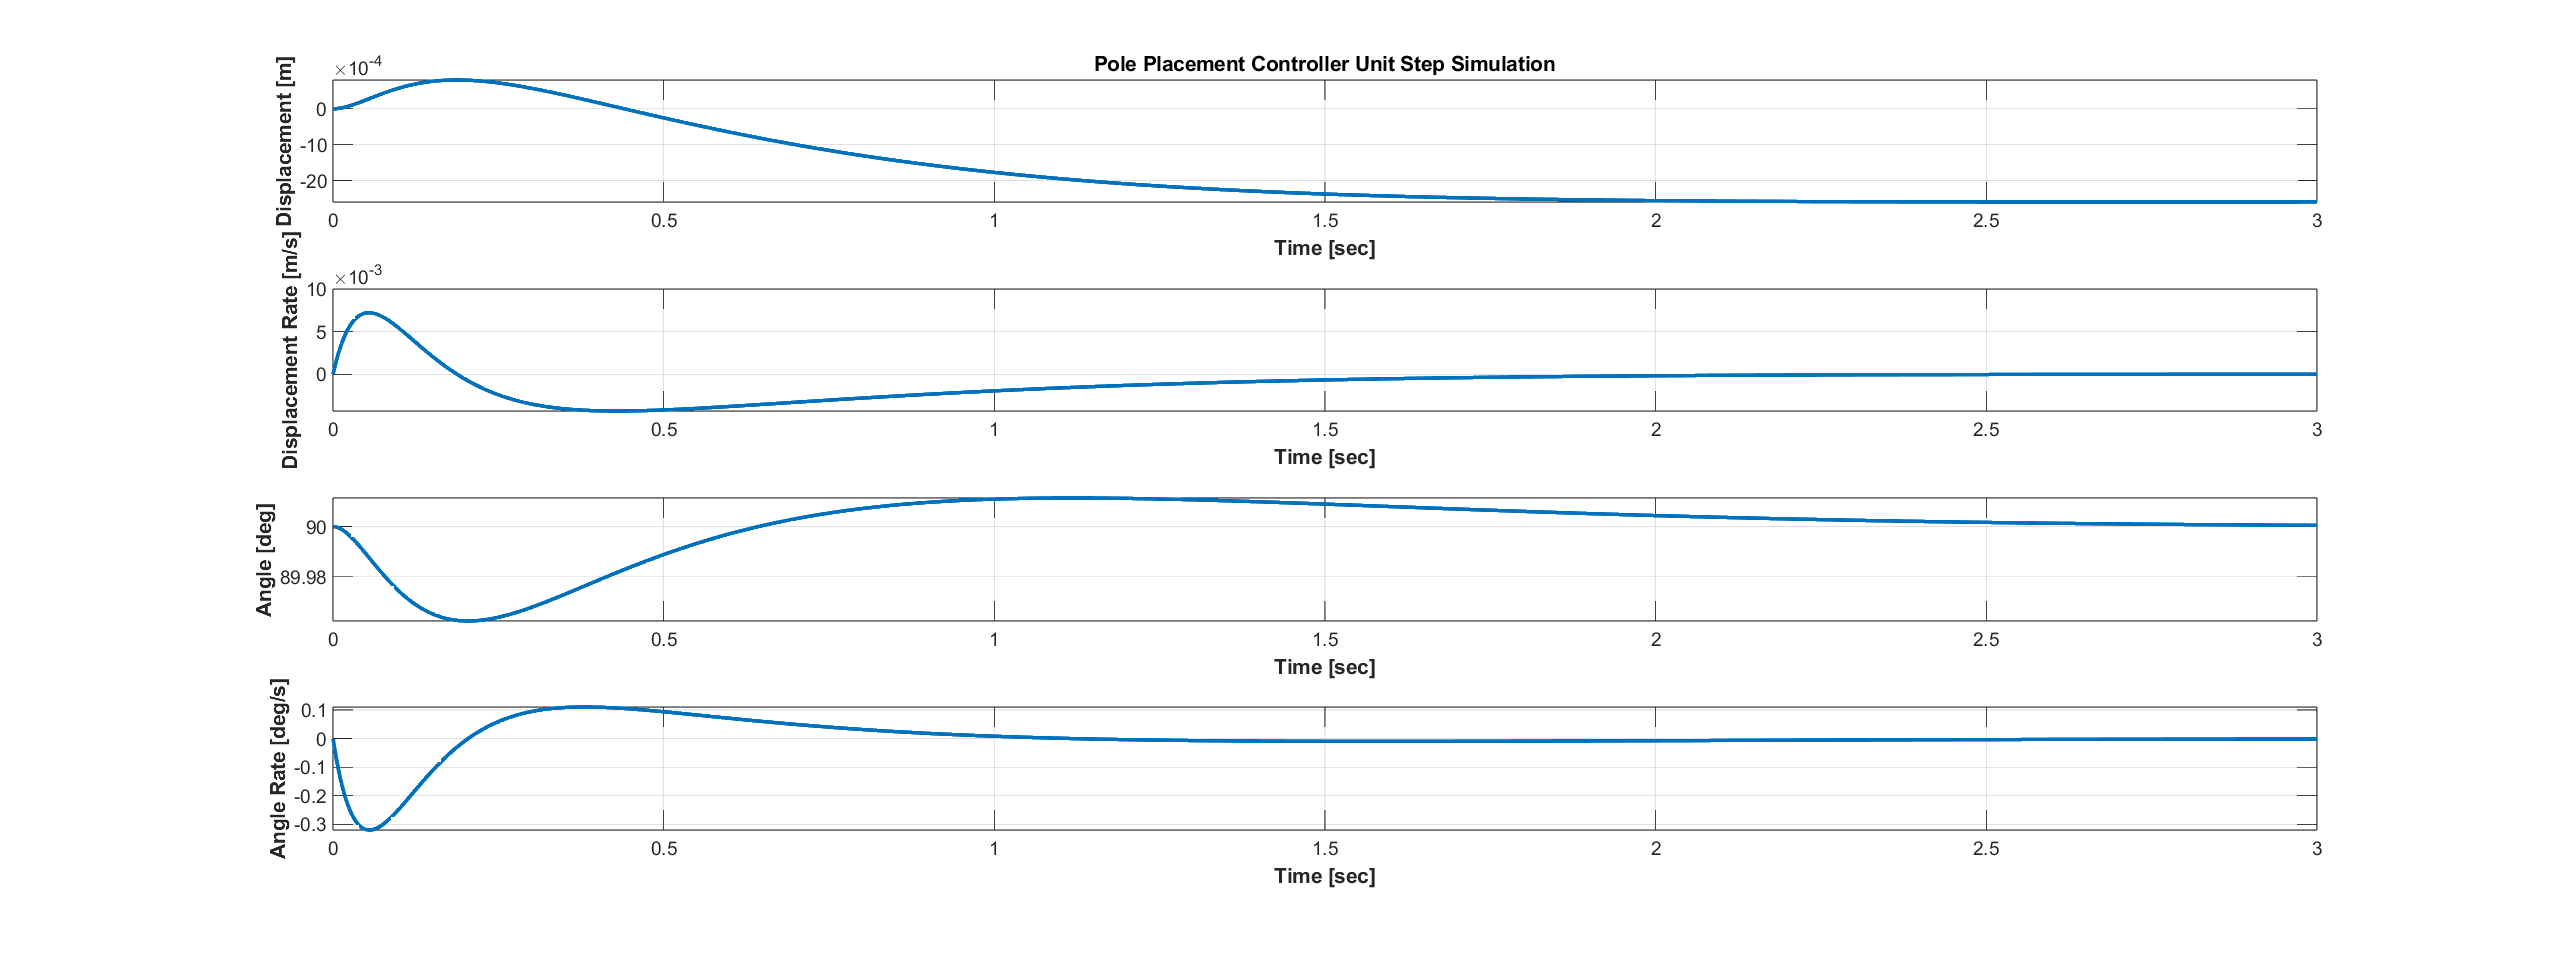
\includegraphics[width=1\linewidth]{pole_placement_unit_step.png}
\caption{Pole Placement Controller Unit Step Disturbance}
\end{figure}

\subsubsection{Unit Impulse Response}
\begin{figure}[H]
\center
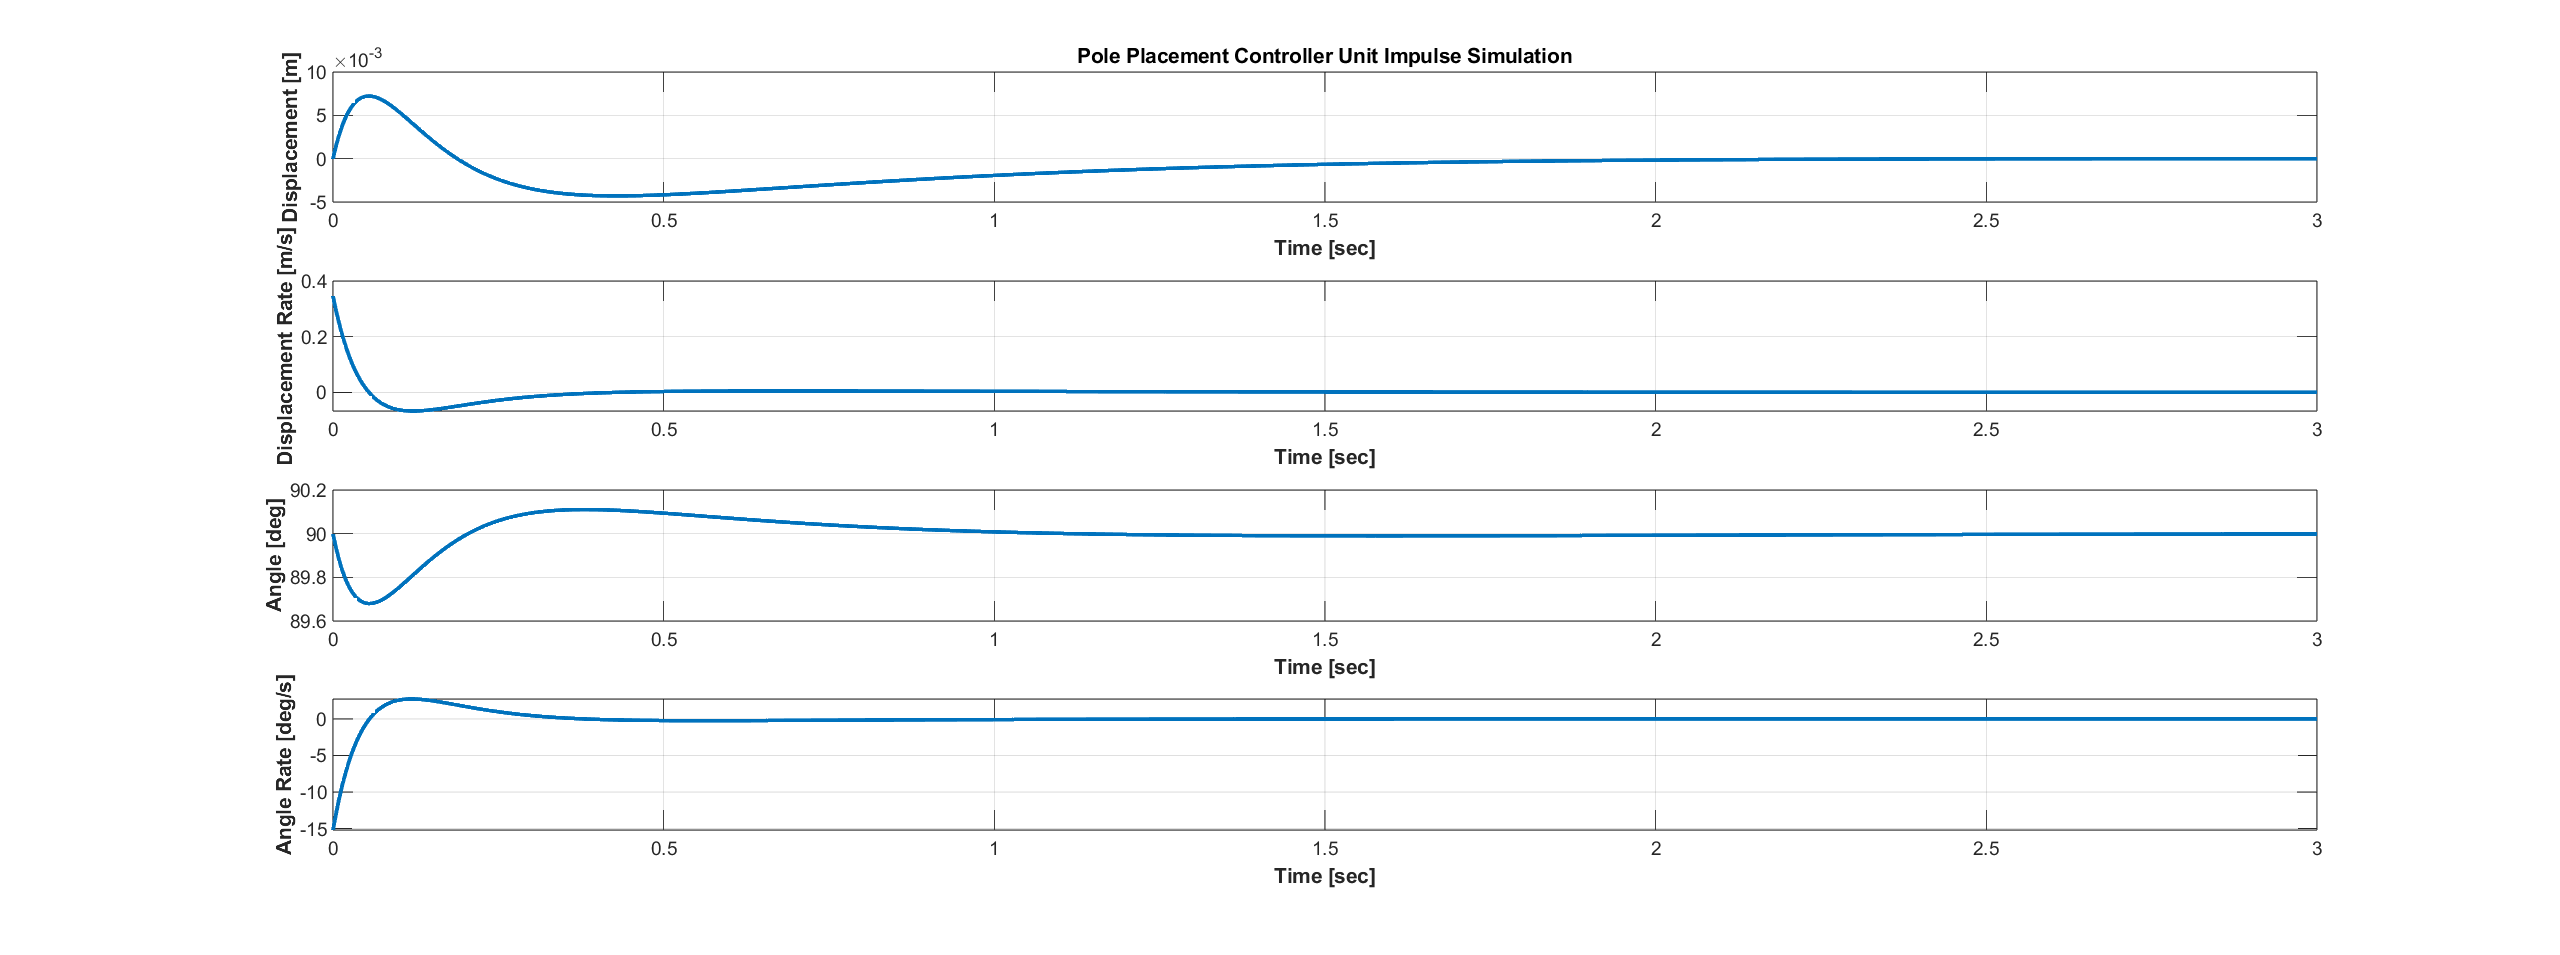
\includegraphics[width=1\linewidth]{pole_placement_unit_impulse.png}
\caption{Pole Placement Controller Unit Impulse Disturbance}
\end{figure}

\subsubsection{Integral Error Controller}

The state feedback controller can be augmented to allow the user to command the cart to a specified position while maintaining the vertical position of the pendulum. To accomplish this, the cart position is fed back and compared against a reference input. The error signal between the user input and the actual position of the cart is used to modify the control input into the system to drive the cart to the commanded position[7, 8].\par

\begin{figure}[h]
    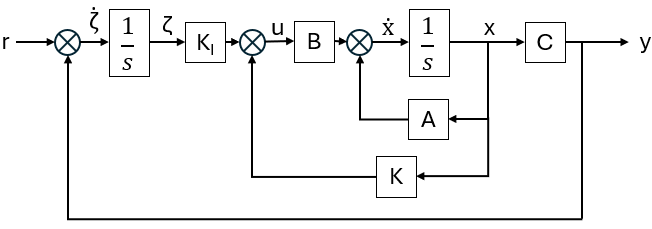
\includegraphics[width=1\linewidth]{cory_controller.png}
    \caption{Integral Error Controller Block Diagram}
    \label{fig:enter-label}
\end{figure}

The system described can be seen in equation (8). Here we can introduce a new state, $\zeta$, which represents the integral of the cart position error. The addition of the integrator ensures that the steady-state error will tend towards zero. The integral error term is modified with a proportional gain $K_I$, and then added to the input signal from the state feedback controller. To derive the appropriate gains using the pole placement method, it is first necessary to modify the states space equations to include the additional state $\zeta$. Referring to figure 8, a new state-space equation can be written as follows[7, 8]:

\begin{equation}
    \begin{bmatrix}
        \mathbf{\dot x(t)} \\
        \boldsymbol{\dot \zeta(t)}
    \end{bmatrix}
    =
    \begin{bmatrix}
        \textbf{A} && \textbf{0} \\
        \textbf{-C} && 0
    \end{bmatrix}
    \begin{bmatrix}
        \textbf{x(t)} \\
        \boldsymbol{\zeta(t)}
    \end{bmatrix}
    +
    \begin{bmatrix}
        \textbf{B} \\ 0
    \end{bmatrix}
    u(t)
    +
    \begin{bmatrix}
        \textbf{0} \\ 1
    \end{bmatrix}
    r(t)
\end{equation}

The steady-state form of the equation can be written as:

\begin{equation}
\begin{bmatrix}
\mathbf{\dot x(\infty)} \\
\boldsymbol{\dot \zeta(\infty)}
\end{bmatrix}
=
\begin{bmatrix}
\textbf{A} && \textbf{0} \\
\textbf{-C} && 0
\end{bmatrix}
\begin{bmatrix}
\boldsymbol{x(\infty)} \\
\boldsymbol{\zeta(\infty)}
\end{bmatrix}
+
\begin{bmatrix}
\textbf{B} \\ 0
\end{bmatrix}
u(\infty)
+
\begin{bmatrix}
\textbf{0} \\ 1
\end{bmatrix}
r(\infty)
\end{equation}

Here x($\infty$), $\zeta(\infty$), and u($\infty$) are the constant steady-state values. If we assume r(t) to be a step input applied at t = 0, then r($\infty$) = r(t) for all t. Using this fact, we can subtract the equation (19) from (20) to eliminate the reference input term and bring us closer to a form that can be used to determine appropriate feedback gain values. Defining new terms, we can come up with the following equations:
\begin{equation}
   \textbf{e} = 
   \begin{bmatrix}
       \mathbf{x(\infty) - x(t)} \\ \boldsymbol{\zeta(\infty)-\zeta(t)}
   \end{bmatrix}   
\end{equation}

\begin{equation}
   u_{e} = u(\infty) - u(t)
\end{equation}

\begin{equation}
    \mathbf{\hat{A}} = 
    \begin{bmatrix}
        \textbf{A} && \textbf{0}\\
        \textbf{-C} && 0
    \end{bmatrix}
\end{equation}

\begin{equation}
    \mathbf{\hat{B}} = 
    \begin{bmatrix}
        \textbf{B}\\
        0
    \end{bmatrix}
\end{equation}

\begin{equation}
    \mathbf{\dot e} = \mathbf{\hat{A}e} + \mathbf{\hat{B}u}
\end{equation}

Now defining the input, $u_e$, as

\begin{equation}
    u_{e} = \mathbf{-K(x(\infty) - x(t))} + K_{I}(\mathbf{\zeta(\infty)-\zeta(t))}
\end{equation}

and

\begin{equation}
    \mathbf{\hat{K}} = 
    \begin{bmatrix}
        \textbf{K} && -K_{I}
    \end{bmatrix}
\end{equation}

we come up with our equation that can be used for finding the feedback gains using the pole placement method.

\begin{equation}
    \mathbf{\dot e} = \mathbf{(\hat{A}-\hat{B}\hat{K)}e}
\end{equation}

The controllability matrix using the new state matrices can be used to determine the controllability for the new system.

\begin{equation}
    \textbf{P} = 
    \begin{bmatrix}
        \textbf{B} && \textbf{AB} && \textbf{A}^2\textbf{B} && \textbf{A}^3\textbf{B} && \textbf{A}^4\textbf{B}
    \end{bmatrix}
\end{equation}

Since the rank of the controllability matrix is 5, the newly formed system is completely state controllable and the pole placement method can be used to determine the feedback gains. These gains were determined by using a fifth-order Bessel polynomial with roots equating to an approximately one second settling time and the pole placement function in MATLAB. The gain values were then incorporated into the following state-space representation of the original system.

\begin{equation}
\begin{bmatrix}
\mathbf{\dot x(t)} \\
\boldsymbol{\dot \zeta(t)}
\end{bmatrix}
=
\begin{bmatrix}
\textbf{A}-\textbf{BK} && \textbf{B}K_{I} \\
-\textbf{C} && 0
\end{bmatrix}
\begin{bmatrix}
\textbf{x} \\
\boldsymbol{\zeta}
\end{bmatrix}
+
\begin{bmatrix}
\textbf{0} \\ 1
\end{bmatrix}
r
\end{equation}

The system was given a unit step input that was equivalent to a cart position of 5 meters. The displacement and pendulum angle response can be seen in the following figures. The cart position is shown to settle at the commanded value of 5 meters after approximately 3 seconds. The system remains stable as the pendulum stabilizes back to its equilibrium position at steady-state.

\begin{figure}[H]
\center
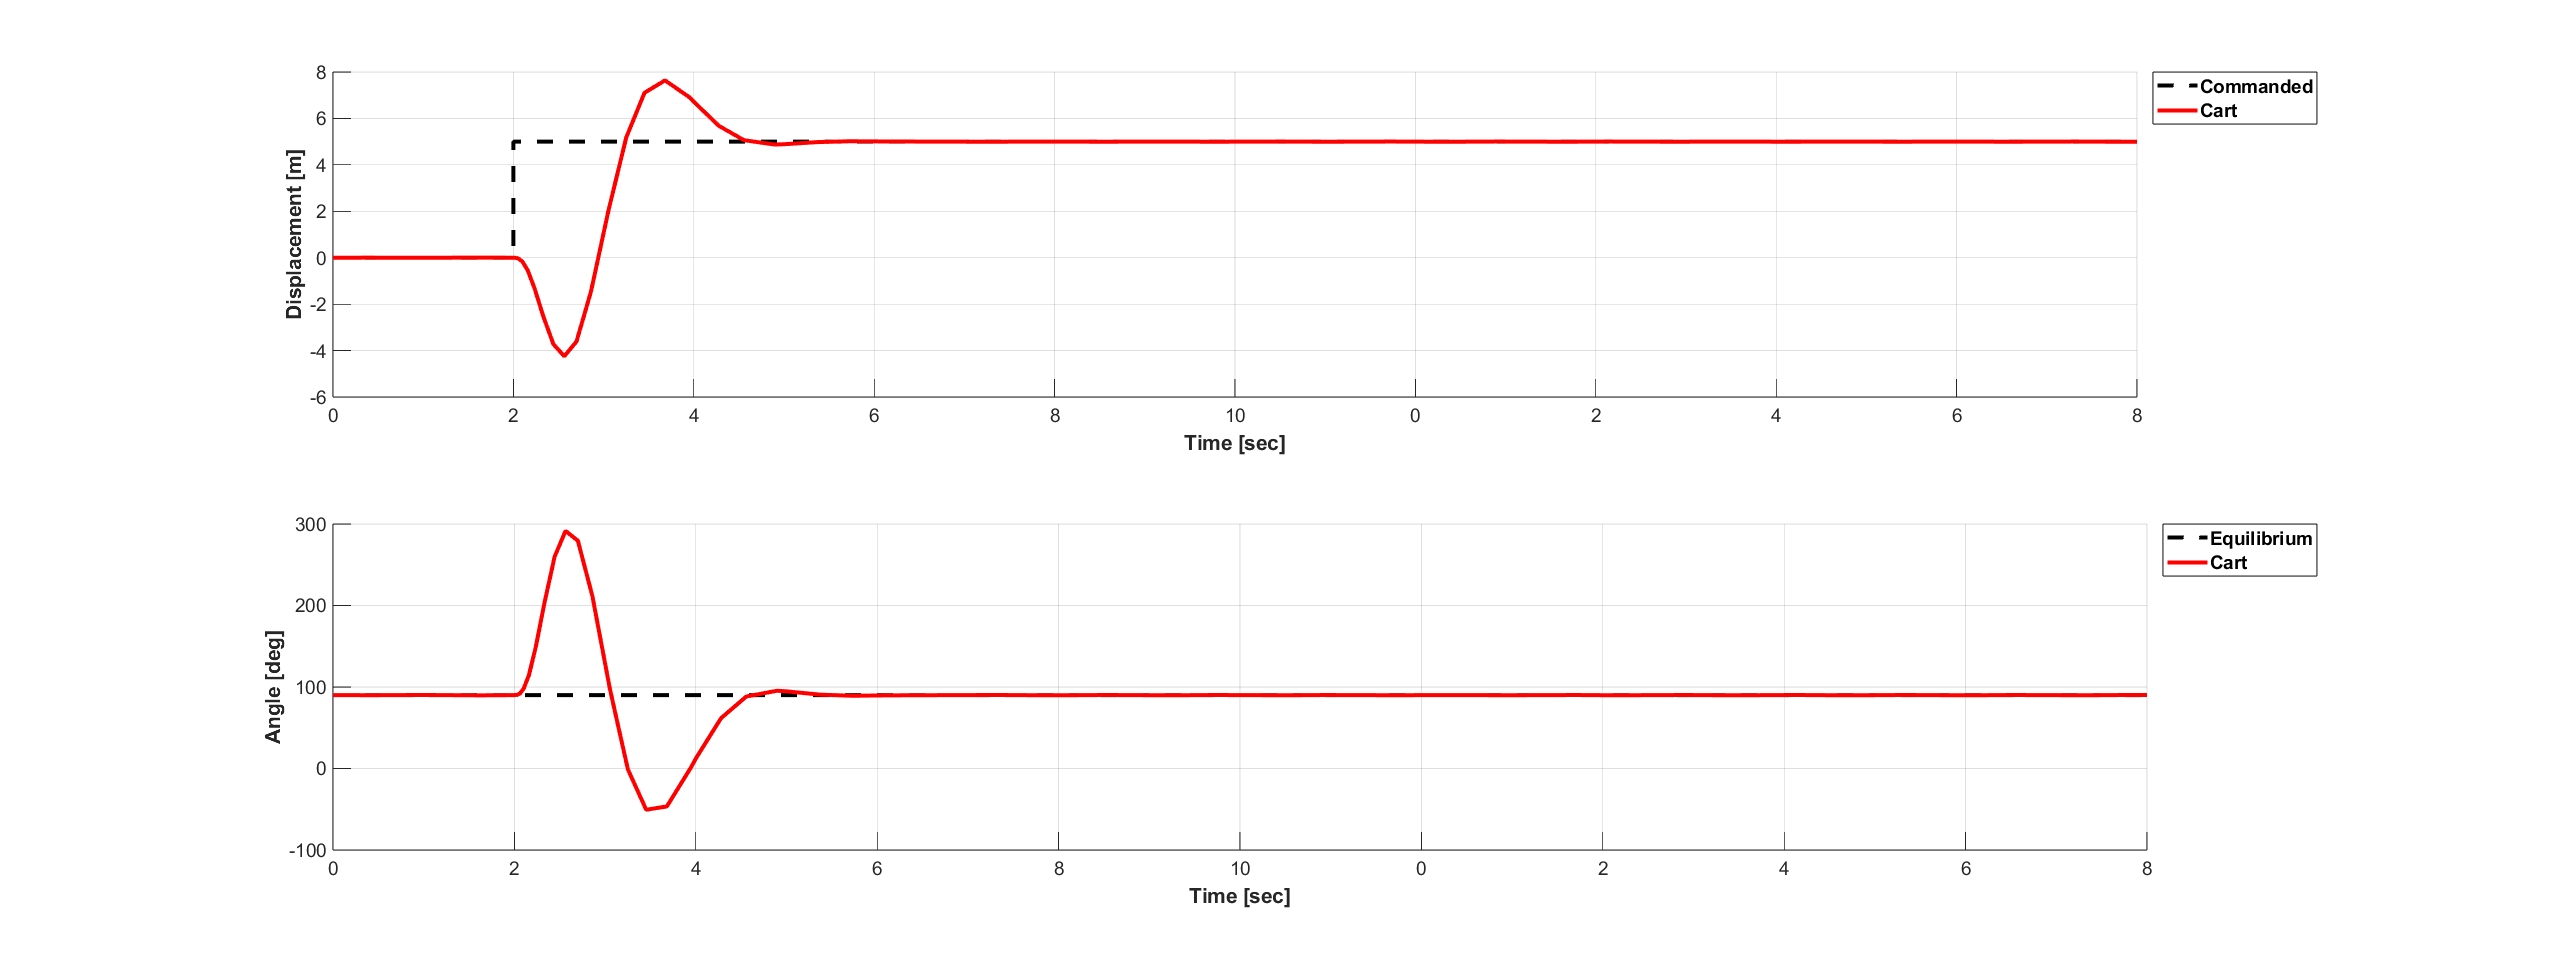
\includegraphics[width=15cm, height=9cm]{pole_placement_integral_error.png}
\caption{Pole Placement Controller Integral Error Control}
\end{figure}

\subsection{LQR}

The concept of LQR, first introduced by Rudolf Kalman in 1960, is a control method that has been successfully applied to many systems. An LQR controller can stabilize an unstable system, such as the inverted pendulum, by minimizing a cost function or performance index, “J”, where[4, 9]:
\begin{equation}
J = \int_{0}^{\infty} \left( -\frac{d}{dt}\left(\vec(x)^{t}\textbf{P}\vec{x}\right)\right)dt = -\vec{x}^{T}\textbf{P}\vec{x}\biggr\rvert_{0}^{\infty}=\vec{x}^{T}\left(0\right)\textbf{P}\vec{x}\left(0\right)
\end{equation}

The \textbf{Q} matrix is a weighting matrix that penalizes deviation from reference states. The \textbf{R} matrix penalizes control effort. Using matrices \textbf{Q} and \textbf{R}, the Riccati equation below can be solved to obtain matrix \textbf{P}[4, 9].

\begin{equation}
\textbf{A}\textbf{P} + \textbf{P}\textbf{A}^{T} – \textbf{P}\textbf{B}^{T}\textbf{R}^{-1}\textbf{B}\textbf{P} + \textbf{Q} = \begin{bmatrix} \textbf{0}\\\end{bmatrix}
\end{equation}

The optimum feedback gain matrix, \textbf{K}, can subsequently be calculated from equation (33)[4, 9]:

\begin{equation}
\textbf{K} = -\textbf{R}^{-1}\textbf{B}^{T}\textbf{P}
\end{equation}

To achieve optimal stability and performance, correct selection of weighting matrices \textbf{Q} and \textbf{R} is essential. The conventional approach is trial and error using knowledge of the system. The higher the order of the system, the more challenging it becomes to correctly assign weights. Optimization techniques have long been investigated by researchers.\\

For this project, it was desired to design the LQR controller based on such research, as opposed to simply using a trial-and-error method. Optimization techniques such as Particle Swarm Optimization, Genetic Algorithms, and Artificial Bee Colony were investigated through paper searches. Ultimately, a research paper by Erkol entitled ‘Linear Quadratic Regulator Design for Position Control of an Inverted Pendulum by Grey Wolf Optimizer (GWO)’ was not only found to be appropriate but also transpired to be a fascinating approach to considering the inverted pendulum problem[3].\\

Per Erkol, the GWO is inspired from the Grey Wolf in nature. In a Grey Wolf pack, there are four levels called Alpha, Beta, Delta and Omega. The Alpha Wolf is the group leader and is the most dominant wolf in the pack. The Alpha may not be the most powerful member of the group but it is the best at managing. The Beta Wolf helps the Alpha and is the second in command. They also give feedback to Alpha about the other wolves. The Delta wolves are responsible for hunting, scouting, sentineling, etc. The Omega wolves are at the end of the hierarchy. They always do as the dominant wolves say. They are the last wolves allowed to eat[3].\\

A mathematical model of the wolf pack social hierarchy and hunting behavior, along with the search, encircling and attacking strategy, allows a GWO algorithm to be created. Through successful implementation of the GWO to the inverted pendulum problem, Erkol created the following weighted matrices[3]:

\begin{equation}
		\textbf{Q}=\begin{bmatrix}
			3.471E6 & 0 & 0 & 0\\
			0 & 4.91E3 & 0 & 0\\
			0 & 0 & 3.54E-4 & 0\\
			0 & 0 & 0 & 1.11E4\\
		\end{bmatrix}
		\quad\quad\quad\textbf{R} =
		\begin{bmatrix}
			8779.759
		\end{bmatrix}
\end{equation}

Although the parameters of Erkol’s system did not perfectly match those assigned in this project, Erkol’s \textbf{Q} and \textbf{R} matrices were used to good effect. This selection in both \textbf{Q} and \textbf{R} yield the results in the following section for a unit step and unit impulse. Then in the final section, the LQR controller is compared to the pole placement method controller for a larger perturbation.

	Below is a snippet of the code used to compute the \textbf{K} gain matrix using MATLAB:
	\begin{lstlisting}[style=Matlab-editor]
		%% LQR Controller
		lqr_q_mat = zeros(4);

		% Grey Wolf Optimizer
		lqr_q_mat(1, 1) = 3.471E6;
		lqr_q_mat(2, 2) = 4.91E3;
		lqr_q_mat(3, 3) = 3.54E-4;
		lqr_q_mat(4, 4) = 1.11E4;

		lqr_r = 8779.759;

		[lqr_gain, lqr_s, lqr_poles] = lqr(A, B, lqr_q_mat, lqr_r);

		closeLoopSysLqr = ss(A-B*lqr_gain, B, C, D);
	\end{lstlisting}

\subsubsection{Unit Step Response}

\begin{figure}[H]
\center
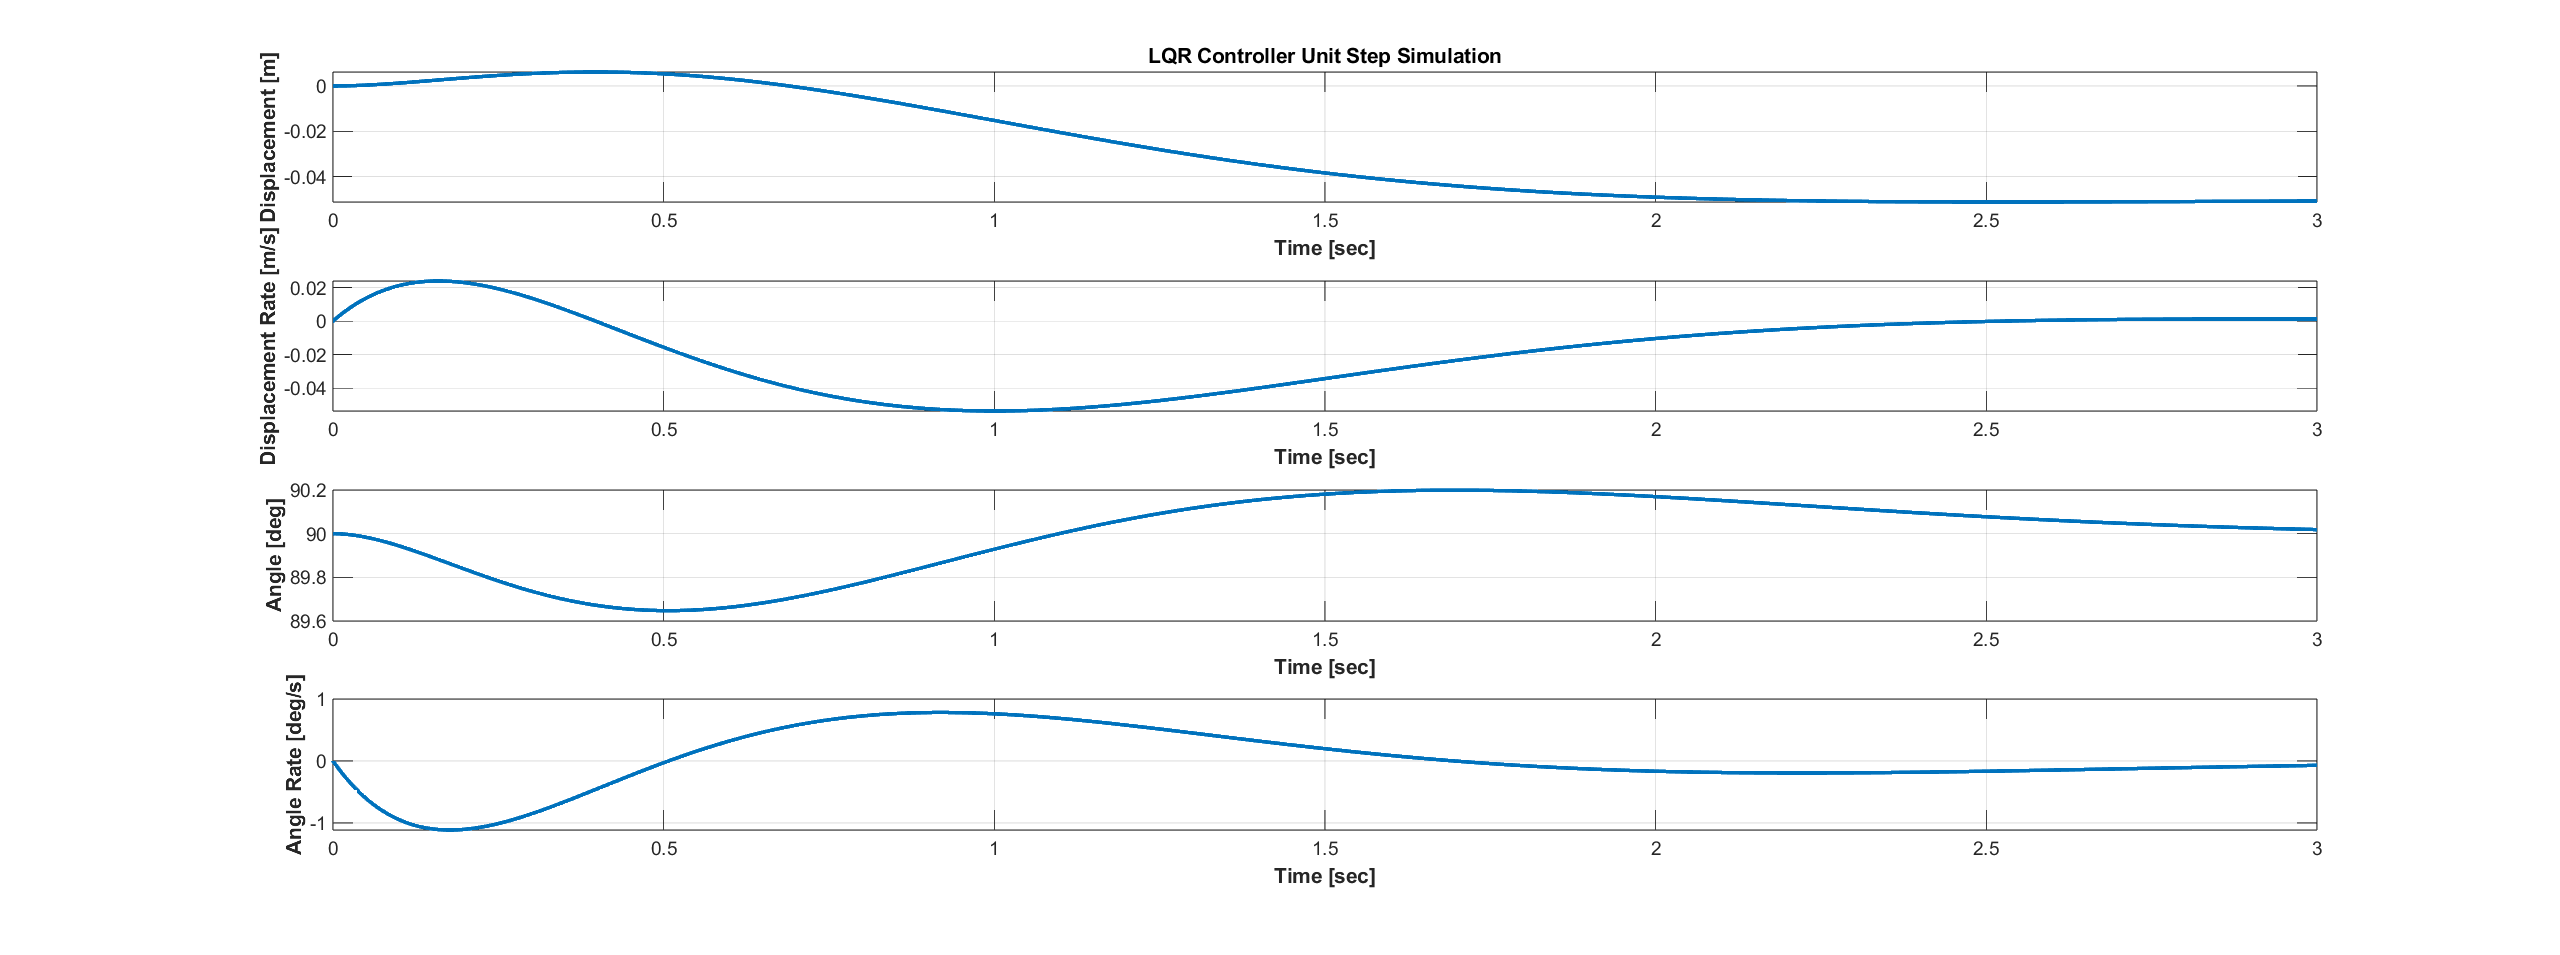
\includegraphics[width=16cm, height=8cm]{lqr_unit_step.png}
\caption{LQR Controller Unit Step Disturbance}
\end{figure}

\subsubsection{Unit Impulse Response}

\begin{figure}[H]
\center
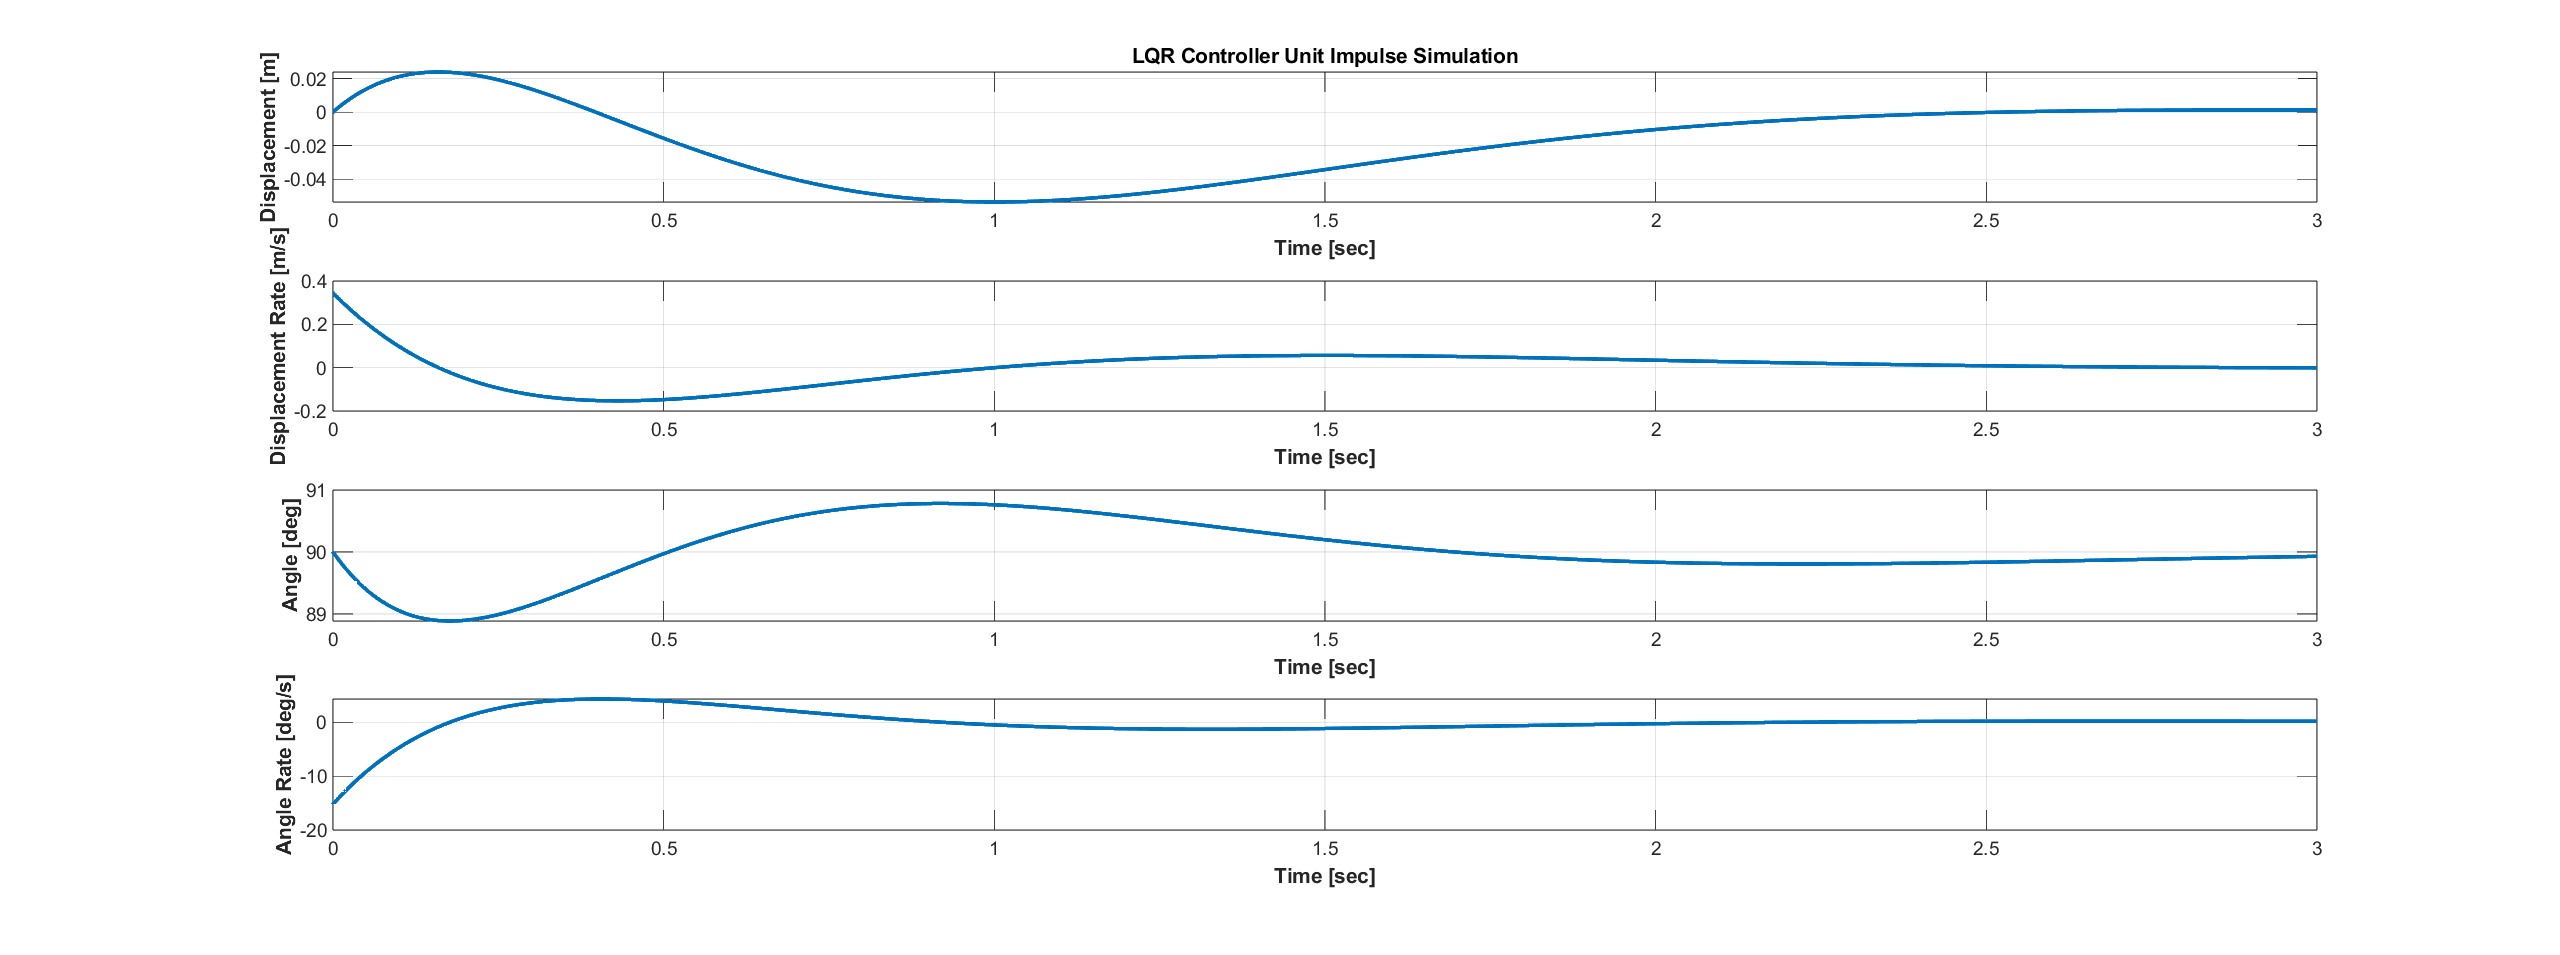
\includegraphics[width=16cm, height=8cm]{lqr_unit_impulse.png}
\caption{LQR Controller Unit Impulse Disturbance}
\end{figure}

\newpage
\section{Response Analysis}

\subsection{Low Frequency Sinusoid Response}
To test the robustness of these controller designs we simulated the response of the system to a low frequency sinusoidal input with an amplitude of 100  and a frequency of 100 Hz .
The results of this simulation can be seen in the following figures.

\begin{figure}[h]
    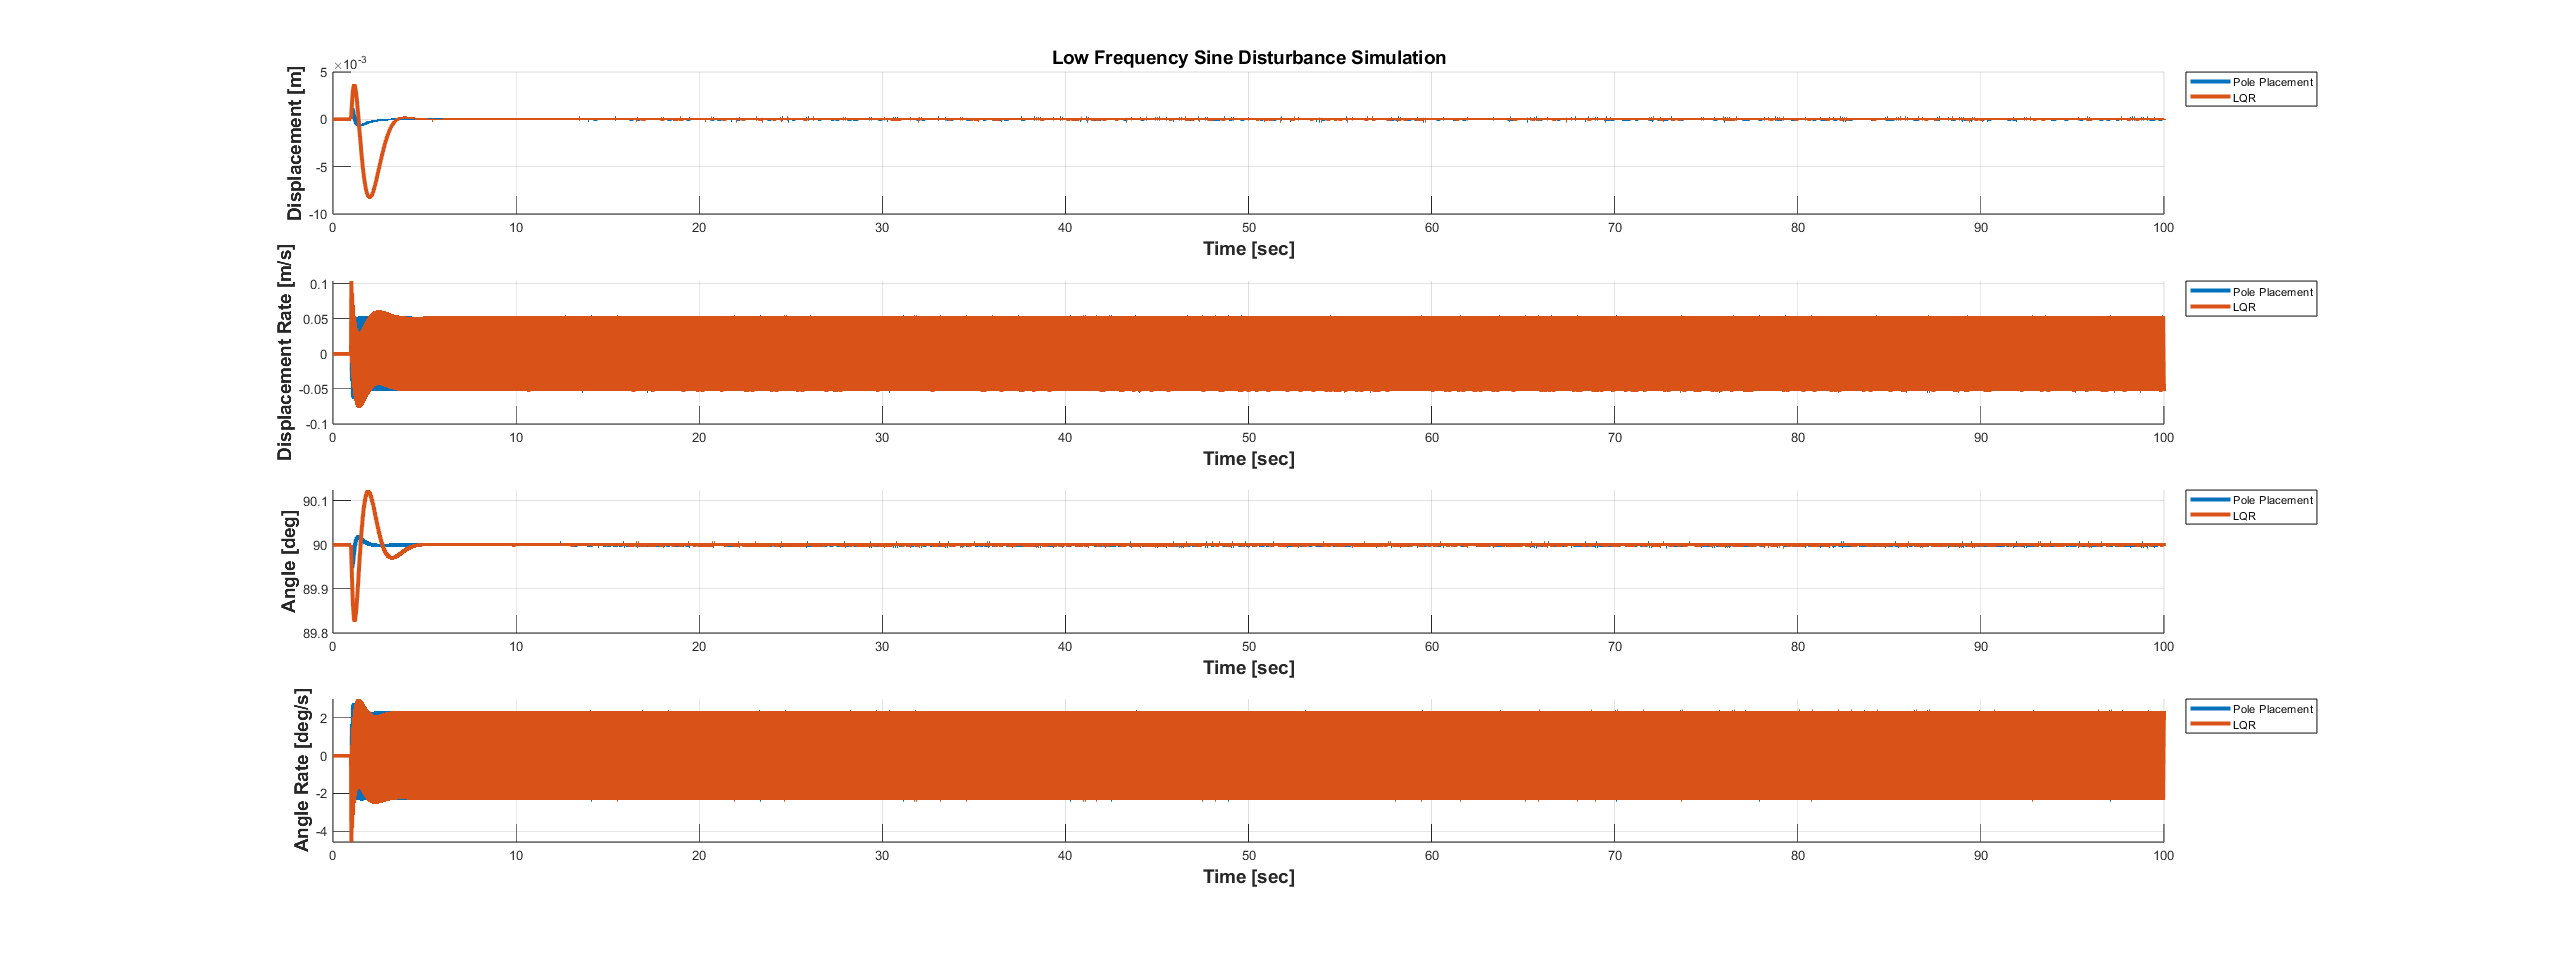
\includegraphics[width=1\linewidth]{low_frequency_sine.png}
    \caption{Low Frequency Sinusoidal Response}
    \label{fig:enter-label}
\end{figure}

\begin{figure}[h]
    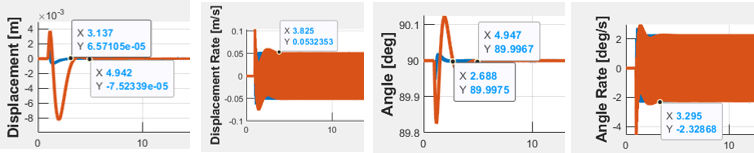
\includegraphics[width=1\linewidth]{eddie_fig_1.png}
    \caption{Low Frequency Sinusoidal Response}
    \label{fig:enter-label}
\end{figure}

These figures show that while these controllers were not specifically designed to handle a sinusoidal input, they are robust enough to stabilize the system. The settling time for the pendulum arm to achieve asymptotic stability at the unstable equilibrium point of 90° was slightly slower, but still within the same ~2–4 second timeframe demonstrated by these controllers when impulse, step, and ramp inputs were introduced. The system was also able to achieve asymptotic stability for cart displacement in the same ~3–5 second timeframe as when impulse and step inputs were introduced but was once again slightly slower. Also, the system was able to stabilize without introducing the displacement creep present when a ramp input is applied.\\

However, these controllers were only able to achieve marginal stability for both displacement rate and angular rate. This finding is logical as periodic adjustments to these states are necessary to offset the effects of the periodic sinusoidal input function.  Marginal stability for these states was achieved slightly slower than asymptotic stability was achieved for impulse and ramp inputs but were slightly faster than when a step input was applied, with all systems reaching stability in ~1.5–5 seconds. The displacement rate for the cart was roughly bounded between 0.053 m/s and -0.053 m/s while angular rate for the pendulum arm was bounded between 2.34 deg/s and -2.34 deg/s for both controllers.\\

\subsection{High Frequency Sinusoid Response}

To test the limits of these controllers we simulated the response of the system to a high frequency sinusoidal input with an amplitude of 100  and a frequency of 1000 Hz . The results of this simulation can be seen in Figure 10.

\begin{figure}[h]
    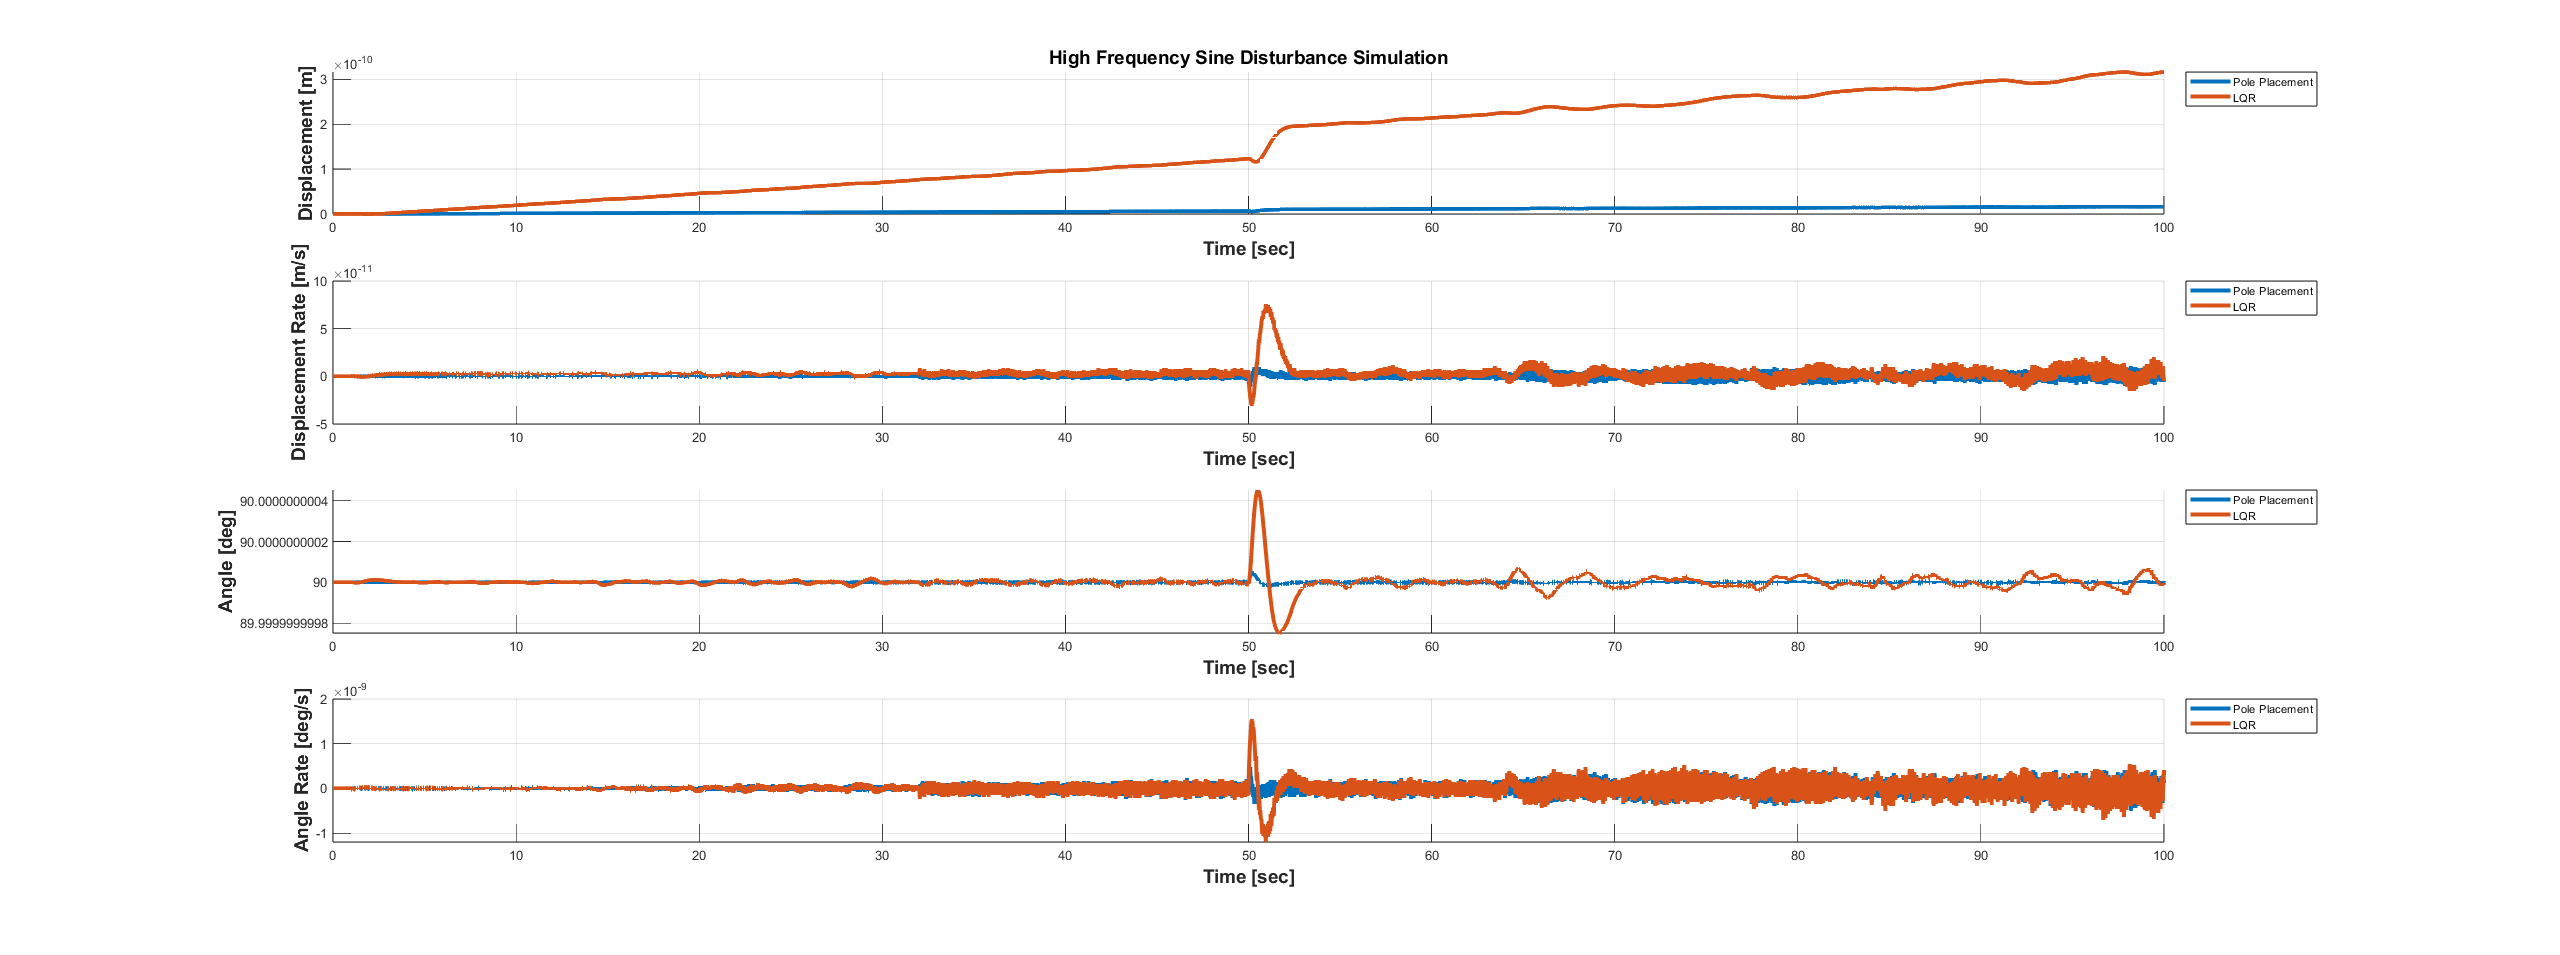
\includegraphics[width=1\linewidth]{high_freq_sine.png}
    \caption{Low Frequency Sinusoidal Response}
    \label{fig:enter-label}
\end{figure}

This figure shows that the controllers had more difficulty stabilizing the system with a high frequency input, especially the LQR controller. The high oscillation rate of the input signal did not trigger a significate controller response until roughly 50 seconds after the simulation began, likely due to it taking that long for the input to induce a large enough harmonic disturbance to require a significate controller response.  Before this event, the controllers only reacted with small response signals which did not stabilize the system and induced displacement creep in the LQR controlled system. After this event the pole placement controller showed relatively strong performance by asymptotically stabilizing the cart displacement and pendulum angle positions in ~2 seconds, slightly faster than its performance with impulse and step inputs and it did not display the displacement creep introduced by ramp inputs. In contrast, the LQR controller introduced a creep to the cart displacement state variable and only achieved marginal stability for the pendulum arm angle position after ~27 seconds  and displayed a complex harmonic  response. However, the amplitude of this harmonic response was less than 1E-10 degrees.\\

Both controllers were only capable of achieving predominantly marginally stable displacement rates and angular rates, which again is logical for this scenario. The displacement rate and angular rate response of the pole placement controller stabilized in ~2 seconds, similar to the responses of this controller to impulse, step, and ramp inputs, however these responses now displayed complex harmonic frequencies. The LQR controller stabilized in ~3 seconds for the displacement rate and angular rate, also similar to its response to impulse, step, and ramp inputs, but with harmonic response frequencies mirroring the angle position response. The displacement rate for the cart with the pole placement controller was roughly bounded between 10.9*E-12 m/s and -8.93*E-12 m/s. However, upon inspection the bounds of the pole placement controller’s angular rate and the LQR controller’s displacement rate and angular rate showed a slight increase in magnitude overtime, indicating instability. The increase was significantly small; ~5.3E-12 for the pole placement controller angular rate, ~3E-12 for the LQR displacement rate, ~2.2E-10 for the LQR angular rate, but was still present. Indicating that with enough time the controller would not be able to stabilize the system.

\newpage
\section{Conclusion}
In conclusion, this project covers the classic control system of an inverted pendulum on a cart. The pendulum is free to rotate around its pivot point while the cart is free to traverse on its axis of travel. The desired position, and equilibrium condition of the system, is for the pendulum to be vertical. The cart is also allowed to move freely and in two of the three controllers its final position is not constrained. However, we implemented a controller that drives the cart to a final displacement and successfully demonstrated that capability in controlling the system. After the dynamical system was derived and linearized three controllers were designed. Two of the controllers used two different methods by placing poles to yield a closed-loop system. The final controller that was designed was a Linear Quadratic Regulator using the Gray Wolf Optimizer to choose the \textbf{Q} and \textbf{R} matrices. Each of these three controllers were initially designed using a unit step and unit impulse function. Once the controller met design criteria with those two inputs, further analysis was conducted to stress the system. The stressing inputs to the system were a ramp function, low frequency sinusoid and high frequency sinusoid. The ramp function results were omitted for brevity. The results from the two sinusoid inputs showed that they were not a strong function of the amplitude and need a large amplitude to get a decent response to the system. However, the frequency did drive the controller response. It was interesting to see that the periodic nature of the perturbation caused a small oscillation around the equilibrium condition yielding that the controllers did not demonstrate asymptotic stability for this equilibrium condition.

\newpage
\section{Appendix A: Source Code}
% Cut and past matlab code here when its all done.
\begin{lstlisting}[style=Matlab-editor]
% Main script for ME 577 Group Final Project
close all; clear; clc;

%% User Inputs
% Initial Conditions
ICs = [0; 0; deg2rad(0); 0];

% Controller Design Parameter: Percent Overshoot
desPO = 10;

% Controller Design Parameter: Settling Time
tSettle = 1;

% Controller Design Parameter: Steady State Metric
inputPercent = 2;

% Controller Design Parameter: Pole Placement Scalar Multiplier
poleScalarOne = 5;
poleScalarTwo = 10;

% Sim Time Vector
timeVec = 0:1E-3:100;

%% System Response Parameters
% Pole Placement and LQR Knobs
pertTime = 1;
stepAmp = 100;
nonUnitImpulseAmp = 100;
sineAmp = 100;
sineFreqLow = 100;
sineFreqHigh = 1000;

%% System Definition -- Constants
m = 0.35;
M = 2.2;
L = 1.3;
b = 0.25;
g = 9.8;

shift = [0, 0, pi/2, 0];

%% Linear EOM Simulation - Newtonian Dynamics Model
A = zeros(4);
A(1,2) = 1;
A(2,2) = (b)./((2*m)+M);
A(2,3) = (m*g)./((2*m)+M);
A(3,4) = 1;
A(4,2) = (-1.*b)./(L.*((2*m)+M));
A(4,3) = (g./L) - ((m*g)./((2*m)+M));

% B Matrix
B = zeros(4,1);
B(2,1) = (1)./((2*m)+M);
B(4,1) = (-1)./(L.*((2*m)+M));

% C Matrix
C = eye(4);

% D Matrix
D = zeros(4, 1);

% % Create a Matlab State Space Model
linSys = ss(A,B,C,D);

%%  Initial Conditions Simulation
[yInitial, tInitial] = initial(linSys, ICs, timeVec);
yInitial = moveOutput(yInitial, shift);
plotStates(yInitial, tInitial, 'Uncontrolled Initial Conditions Simulation');

%%  Unit Step Input Simulation
[yStep, tStep] = step(linSys, timeVec);
yStep = moveOutput(yStep, shift);
plotStates(yStep, tStep, 'Uncontrolled Unit Step Simulation');

%%  Unit Impulse Input Simulation
[yImpulse, tImpulse] = impulse(linSys, timeVec);
yImpulse = moveOutput(yImpulse, shift);
plotStates(yImpulse, tImpulse, 'Uncontrolled Unit Impulse Simulation');

%% Stability -> HW 4 type of analysis
[eigVectors, eigValues] = eig(A);
linSysPole = pole(linSys);

%% Controlability -> HW 5 type of analysis
P = [B, A*B, A*A*B, A*A*A*B];
rankOfP = rank(P);

%% Observability -> HW 5 type of analysis
Q = [C;...
    C*A;...
    C*A*A;...
    C*A*A*A];
rankOfQ = rank(Q);

%% Pole Placement
zeta = (-1*log(desPO./100))/(sqrt((pi.^2) + (desPO./100)));
wn = (-1*log(inputPercent./100))./(tSettle.*zeta);
eqn = [1, 2.1, 3.4, 2.7.*wn, wn.^2];
p = roots(eqn);
stableP = p(real(p) == min(real(p)));
p = [stableP(1); stableP(2);...
    floor(poleScalarOne*min(real(stableP)));...
    floor(poleScalarTwo*min(real(stableP)))];

[K, prec] = place(A, B, p);
closeLoopA = A - (B*K);
closeLoopSysPolePlace = ss(closeLoopA, B, C, D);

%% Pole Placement Controller Design Plots
% Unit Step Input Simulation
[yStepPole, tStepPole] = step(closeLoopSysPolePlace, timeVec);
yStepPole = moveOutput(yStepPole, shift);
plotStates(yStepPole, tStepPole, 'Pole Placement Controller Unit Step Simulation');

%  Unit Impulse Input Simulation
[yImpulsePole, tImpulsePole] = impulse(closeLoopSysPolePlace, timeVec);
yImpulsePole = moveOutput(yImpulsePole, shift);
plotStates(yImpulsePole, tImpulsePole, 'Pole Placement Controller Unit Impulse Simulation');

%% Simulink -- Integral Error Control
% Define new A and B matrices
cIEC = [1 0 0 0];
Ahat = [A zeros(length(A),1); -cIEC 0];
Bhat = [B; 0];

% Check controllabilty of new system. Rank = 5 means that thes system
% is % fully state controllable.
P = [A, B; -cIEC, 0];
rank(P);

% Define desired eigenvalues for new 5th order system. Eigenvalues were
% defined from values that result in a 1 second settling time
eigDesired = [-6.4480,-4.1104+6.3142i,-4.1104-6.3142i,...
    -5.9268+3.0813i,-5.9268-3.0813i];

% Use place command to calculate gain matrix to acheive desired poles
gainMatrix = place(Ahat,Bhat,eigDesired);

% State feedback gain matrix
K = gainMatrix(1:4);

% Integral error tracking gain value
KI = -gainMatrix(5);

% Define desired cart position
cartPosition = 5;

% Define periodic input disturbance amplitude and frequency
periodicDisturbanceAmp = 100;
periodicDisturbanceFreq = 10;

% Define impulse input disturbance amplitude
impulseAmp = 0;

% Run Simulink model
out = sim('stateFeedbackIntegralControl.slx');
intErrPlot(out);

%% LQR Controller
lqr_q_mat = zeros(4);

% Grey Wolf Optimizer
lqr_q_mat(1, 1) = 3.471E6;
lqr_q_mat(2, 2) = 4.91E3;
lqr_q_mat(3, 3) = 3.54E-4;
lqr_q_mat(4, 4) = 1.11E4;

lqr_r = 8779.759;

[lqr_gain, lqr_s, lqr_poles] = lqr(A, B, lqr_q_mat, lqr_r);

closeLoopSysLqr = ss(A-B*lqr_gain, B, C, D);

%% LQR Controller Design Plots
[yStepLqr, tStepLqr] = step(closeLoopSysLqr, timeVec);
yStepLqr = moveOutput(yStepLqr, shift);
plotStates(yStepLqr, tStepLqr, 'LQR Controller Unit Step Simulation');

[yImpulseLqr, tImpulseLqr] = impulse(closeLoopSysLqr, timeVec);
yImpulseLqr = moveOutput(yImpulseLqr, shift);
plotStates(yImpulseLqr, tImpulseLqr, 'LQR Controller Unit Impulse Simulation');

%% System Response Analysis
% Non Unit Impulse
nonUnitImp = genImpulseInput(timeVec, nonUnitImpulseAmp, pertTime);
[yImpPole, tImpPole] = lsim(closeLoopSysPolePlace, nonUnitImp, timeVec);
yImpPole = moveOutput(yImpPole, shift);
[yImpLqr, tImpLqr] = lsim(closeLoopSysLqr, nonUnitImp, timeVec);
yImpLqr = moveOutput(yImpLqr, shift);

% Non Unit Step
nonUnitStep = genStepInput(timeVec, stepAmp, pertTime);
[yStepPole, tStepPole] = lsim(closeLoopSysPolePlace, nonUnitStep, timeVec);
yStepPole = moveOutput(yStepPole, shift);
[yStepLqr, tStepLqr] = lsim(closeLoopSysLqr, nonUnitStep, timeVec);
yStepLqr = moveOutput(yStepLqr, shift);

% Ramp
ramp = genRampInput(timeVec, pertTime);
[yRampPole, tRampPole] = lsim(closeLoopSysPolePlace, ramp, timeVec);
yRampPole = moveOutput(yRampPole, shift);
[yRampLqr, tRampLqr] = lsim(closeLoopSysLqr, ramp, timeVec);
yRampLqr = moveOutput(yRampLqr, shift);

% low freq sine
lowFreqSine = genSinusodialInput(timeVec, pertTime, sineAmp, sineFreqLow);
[ySinePole, tSinePole] = lsim(closeLoopSysPolePlace, lowFreqSine, timeVec);
ySinePole = moveOutput(ySinePole, shift);
[ySineLqr, tSineLqr] = lsim(closeLoopSysLqr, lowFreqSine, timeVec);
ySineLqr = moveOutput(ySineLqr, shift);

% high freq sine
highFreqSine = genSinusodialInput(timeVec, pertTime, sineAmp, sineFreqHigh);
[ySinePole2, tSinePole2] = lsim(closeLoopSysPolePlace, highFreqSine, timeVec);
ySinePole2 = moveOutput(ySinePole2, shift);
[ySineLqr2, tSineLqr2] = lsim(closeLoopSysLqr, highFreqSine, timeVec);
ySineLqr2 = moveOutput(ySineLqr2, shift);

%% System Response Analysis Plots
genMultiPlot(tImpPole, yImpPole, 'Pole Placement',...
    tImpLqr, yImpLqr, 'LQR', 'Non-Unit Impulse Disturbance Simulation')
genMultiPlot(tStepPole, yStepPole, 'Pole Placement',...
    tStepLqr, yStepLqr, 'LQR', 'Non-Unit Step Disturbance Simulation')
genMultiPlot(tRampPole, yRampPole, 'Pole Placement',...
    tRampLqr, yRampLqr, 'LQR', 'Ramp Disturbance Simulation')
genMultiPlot(tSinePole, ySinePole, 'Pole Placement',...
    tSineLqr, ySineLqr, 'LQR', 'Low Frequency Sine Disturbance Simulation')
genMultiPlot(tSinePole2, ySinePole2, 'Pole Placement',...
    tSineLqr2, ySineLqr2, 'LQR', 'High Frequency Sine Disturbance Simulation')

%% Helper Functions
function [y] = moveOutput(y, shift)
    for ii = 1:1:size(y, 1)
        y(ii, :) = y(ii, :) + shift;
    end
end

function [] = plotStates(y, t, titleString)
    figure()
    subplot(4, 1, 1)
    plot(t, y(:, 1), 'Linewidth', 3)
    grid on
    xlabel('Time [sec]', 'fontweight', 'bold', 'fontsize', 14)
    ylabel('Displacement [m]', 'fontweight', 'bold', 'fontsize', 14)
    title(titleString, 'fontweight', 'bold', 'fontsize', 14)
    a = get(gca,'XTickLabel');
    set(gca,'XTickLabel', a,'fontsize', 14)
    
    subplot(4, 1, 2)
    plot(t, y(:, 2), 'Linewidth', 3)
    grid on
    xlabel('Time [sec]', 'fontweight', 'bold', 'fontsize', 14)
    ylabel('Displacement Rate [m/s]', 'fontweight', 'bold', 'fontsize', 14)
    a = get(gca,'XTickLabel');
    set(gca,'XTickLabel', a,'fontsize', 14)

    subplot(4, 1, 3)
    plot(t, rad2deg(y(:, 3)), 'Linewidth', 3)
    grid on
    xlabel('Time [sec]', 'fontweight', 'bold', 'fontsize', 14)
    ylabel('Angle [deg]', 'fontweight', 'bold', 'fontsize', 14)
    a = get(gca,'XTickLabel');
    set(gca,'XTickLabel', a,'fontsize', 14)
    
    subplot(4, 1, 4)
    plot(t, rad2deg(y(:, 4)), 'Linewidth', 3)
    grid on
    xlabel('Time [sec]', 'fontweight', 'bold', 'fontsize', 14)
    ylabel('Angle Rate [deg/s]', 'fontweight', 'bold', 'fontsize', 14)
    a = get(gca,'XTickLabel');
    set(gca,'XTickLabel', a,'fontsize', 14)
end

function [] = intErrPlot(out)
    figure()
    subplot(2, 1, 1)
    hold on
    plot(out.tout,out.command,'--k', 'Linewidth', 3)
    plot(out.tout,out.position,'-r', 'Linewidth', 3)
    hold off
    grid on
    legend("Commanded","Cart", 'fontweight', 'bold', 'fontsize', 14, 'Location',...
        'BestOutside')
    xlabel('Time [sec]', 'fontweight', 'bold', 'fontsize', 14)
    ylabel('Displacement [m]', 'fontweight', 'bold', 'fontsize', 14)
    a = get(gca,'XTickLabel');
    set(gca,'XTickLabel', a,'fontsize', 14)
    
    subplot(2, 1, 2)
    hold on
    plot(out.tout, 90.*ones(size(out.theta, 1), 1),'--k', 'Linewidth', 3)
    plot(out.tout, rad2deg(out.theta + pi./2),'r', 'Linewidth', 3)
    hold off
    grid on
    legend("Equilibrium","Cart", 'fontweight', 'bold', 'fontsize', 14, 'Location',...
        'BestOutside')
    xlabel('Time [sec]', 'fontweight', 'bold', 'fontsize', 14)
    ylabel('Angle [deg]', 'fontweight', 'bold', 'fontsize', 14)
    a = get(gca,'XTickLabel');
    set(gca,'XTickLabel', a,'fontsize', 14)
end

function [u] = genStepInput(tVec, Amp, stepTime)
    
    u = NaN(size(tVec));

    for ii = 1:1:length(u)
        if tVec(ii) > stepTime
            u(ii) = Amp;
        else
            u(ii) = 0;
        end
    end
end

function [u] = genImpulseInput(tVec, Amp, impulseTime)
    u = NaN(size(tVec));

    for ii = 1:1:length(u)
        if tVec(ii) == impulseTime
            u(ii) = Amp;
        else
            u(ii) = 0;
        end
    end
end

function [u] = genRampInput(tVec, timeShift)
    u = tVec - timeShift;
end

function [u] = genSinusodialInput(tVec, timeShift, amp, freq)
    
    omega = freq .* 2 .* pi;

    u = NaN(size(tVec));

    for ii = 1:1:length(u)
        if tVec(ii) > timeShift
            u(ii) = amp.*sin(omega.*(tVec(ii)-timeShift));
        else
            u(ii) = 0;
        end
    end
end

function [] = genMultiPlot(t1, y1, legend_1, t2, y2, legend_2, titleString)
    figure()
    subplot(4, 1, 1)
    hold on
    plot(t1, y1(:, 1), 'Linewidth', 3)
    plot(t2, y2(:, 1), 'Linewidth', 3)
    grid on
    legend(legend_1, legend_2, 'Location', 'BestOutside')
    xlabel('Time [sec]', 'fontweight', 'bold', 'fontsize', 14)
    ylabel('Displacement [m]', 'fontweight', 'bold', 'fontsize', 14)
    title(titleString, 'fontweight', 'bold', 'fontsize', 14)
    
    subplot(4, 1, 2)
    hold on
    plot(t1, y1(:, 2), 'Linewidth', 3)
    plot(t2, y2(:, 2), 'Linewidth', 3)
    hold off
    grid on
    legend(legend_1, legend_2, 'Location', 'BestOutside')
    xlabel('Time [sec]', 'fontweight', 'bold', 'fontsize', 14)
    ylabel('Displacement Rate [m/s]', 'fontweight', 'bold', 'fontsize', 14)

    subplot(4, 1, 3)
    hold on
    plot(t1, rad2deg(y1(:, 3)), 'Linewidth', 3)
    plot(t2, rad2deg(y2(:, 3)), 'Linewidth', 3)
    hold off
    grid on
    legend(legend_1, legend_2, 'Location', 'BestOutside')
    xlabel('Time [sec]', 'fontweight', 'bold', 'fontsize', 14)
    ylabel('Angle [deg]', 'fontweight', 'bold', 'fontsize', 14)
    
    subplot(4, 1, 4)
    hold on
    plot(t1, rad2deg(y1(:, 4)), 'Linewidth', 3)
    plot(t2, rad2deg(y2(:, 4)), 'Linewidth', 3)
    hold off
    grid on
    legend(legend_1, legend_2, 'Location', 'BestOutside')
    xlabel('Time [sec]', 'fontweight', 'bold', 'fontsize', 14)
    ylabel('Angle Rate [deg/s]', 'fontweight', 'bold', 'fontsize', 14)
end

\end{lstlisting}

\newpage
\section{Appendix B: Simulink}
\begin{figure}[h]
    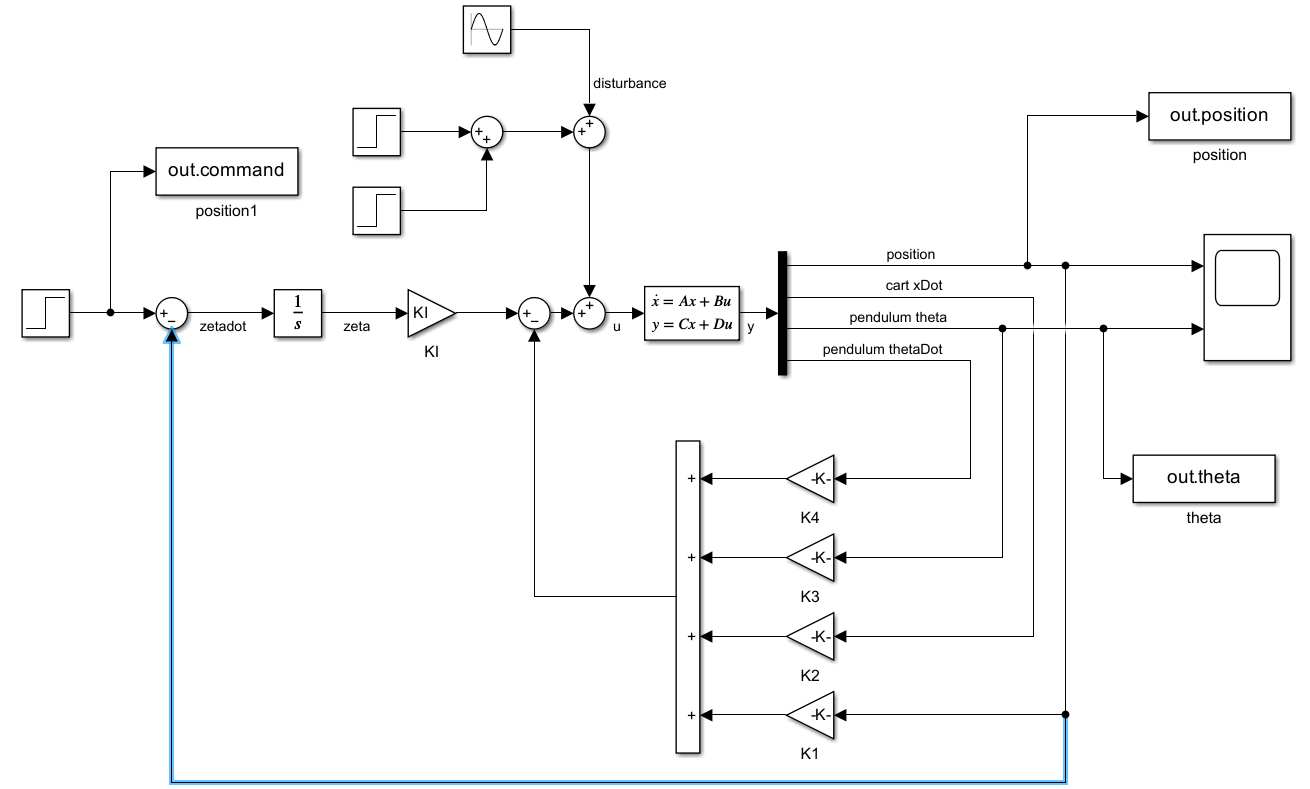
\includegraphics[width=1\linewidth]{simulink_mdl.png}
    \caption{Integral Error Control Simulink Model}
    \label{fig:enter-label}
\end{figure}

\newpage
\section{References}
\begin{enumerate}

\item{Brogan, W., \textit{Modern Control Theory}, 3rd ed., Prentice Hall, Upper Saddle River, NJ, 1991}

\item{Chen, C., \textit{Linear Systems Theory and Design}, 1st ed., Oxford, New York, 1984}

\item{Erkol, H., "Linear Quadratic Regulator Design for Position Control of an Inverted Pendulum by Grey Wolf Optimizer", International Journal of Advanced Computer Science and Applications, Vol 9, No 4, 2018}

\item{Lavretsky, E., \& Wise, K., \textit{Robust and Adaptive Control}, 2nd ed., Springer Nature, Switzerland, 2024}

\item{Pei, J., \& Rothhaar, P., "Demonstration of the Space Launch System Augmenting Adaptive Control Algorithm on Pole-Cart Platform", 2018 AIAA Guidance Navigation, and Control Conference, 8-12 January 2018, Kissimmee, Florida, https://doi.org/10.2514/6.2018-0608}

\item{Schaub, H., \& Junkins, J., "Particle Kinematics",  \textit{Analytical Mechanics of Space Systems}, 3rd ed., AIAA, June 2014, pp. 1-30.}

\item{Zhang, Q., "Lesson 20, Spring 2025", ME 577 University of Alabama, Spring 2025, retrieved: April 2025}

\item{Zhang, Q., "Lesson 21, Spring 2025", ME 577 University of Alabama, Spring 2025, retrieved: April 2025}

\item{Zhang, Q., "Lesson 25, Spring 2025", ME 577 University of Alabama, Spring 2025, retrieved: April 2025}


\end{enumerate}

\end{document}
